\documentclass[conference]{IEEEtran}
\IEEEoverridecommandlockouts
% The preceding line is only needed to identify funding in the first footnote. If that is unneeded, please comment it out.
\usepackage{cite}
\usepackage{amsmath,amssymb,amsfonts}
\usepackage{algorithmic}
\usepackage{graphicx}
\usepackage[normalem]{ulem}
\usepackage{multirow}
\usepackage{longtable}
\usepackage{hyperref}
\usepackage{xltabular}
\usepackage{textcomp}
\usepackage{xcolor}
\def\BibTeX{{\rm B\kern-.05em{\sc i\kern-.025em b}\kern-.08em
    T\kern-.1667em\lower.7ex\hbox{E}\kern-.125emX}}
\begin{document}

\title{Optimal Allocation of Multiple Distributed Generation Using an Enhanced Whale Optimization Algorithm\\
%{\footnotesize \textsuperscript{*}Note: Sub-titles are not captured in Xplore and
%should not be used}
%\thanks{Identify applicable funding agency here. If none, delete this.}
}

\author{\IEEEauthorblockN{John Laurence P. Elambayo}
\IEEEauthorblockA{\textit{Electrical and Electronics Engineering Institute} \\
\textit{University of the Philippines Diliman}\\
Quezon City, Philippines \\
john.laurence.elambayo@eee.upd.edu.ph}
\and
\IEEEauthorblockN{Adonis Emmanuel DC. Tio}
\IEEEauthorblockA{\textit{Electrical and Electronics Engineering Institute} \\
\textit{University of the Philippines Diliman}\\
Quezon City, Philippines \\
adonis.tio@eee.upd.edu.ph}
}
%1\textsuperscript{nd}
\maketitle

\begin{abstract}
The integration of distributed generation (DG) into the distribution system is a complex problem that requires an efficient optimization technique. To maximize benefits while minimizing disadvantages, it is crucial to determine optimal locations and capacities for DG installations. Despite the frequent use of recently developed optimization algorithms, their enhanced counterparts are rarely investigated. Moreover, most research relied on peak loads, which do not accurately reflect real-world demand. We proposed using the enhanced whale optimization algorithm (E-WOA) for optimal DG allocation in a radial distribution system, aiming to minimize power and energy losses. This study also developed representative variable load profiles based on real-world consumption data. The backward/forward sweep algorithm is used for load flow analysis, with the IEEE 33-Bus radial distribution system serving as the test system. The optimization was simulated over 100 independent runs, each with 200 iterations and a population of 50. Results demonstrated that E-WOA effectively solves the optimal DG allocation problem, achieving a power loss of 72.785 kW for three DGs at unity power factor, outperforming the standard WOA and several recent algorithms, and matching the performance of hybrid algorithms. Comparison with WOA across different loading scenarios showed that E-WOA consistently produced higher quality solutions at the cost of slower convergence speeds, longer runtimes, and poor scalability. These suggest E-WOA's limitations in addressing large-scale optimization tasks.
\end{abstract}

\begin{IEEEkeywords}
distributed generation, optimal distributed generation allocation, metaheuristic algorithms, radial distribution system, enhanced whale optimization algorithm


\end{IEEEkeywords}

\section{Background}
The increasing penetration of Distributed Generation (DG) in power systems is a direct response to the numerous challenges in the modern energy landscape. Rising energy demand, environmental concerns, and the necessity for a more resilient and reliable power supply have propelled the widespread adoption of DG technologies. This transition is further driven by declining costs of renewable energy sources, advancements in energy storage solutions, the growing popularity of electric vehicles, increasing fossil fuel prices, and supportive global decarbonization policies \cite{IEA}.

However, integrating DG into power systems can disrupt system dynamics and introduce complications such as reduced system reliability and higher power losses. When properly integrated, DG can offer significant economic benefits, reduced emissions, and other power system advantages. Determining the optimal location and capacity of DG installations through exhaustive brute force methods is feasible for simple, small-scale systems. However, for larger, more complex systems, these methods become computationally expensive, inefficient, and time-consuming.

To address this, many studies have applied intelligent search or metaheuristic algorithms to the optimal DG allocation (ODGA) problem. These algorithms provide more adaptive, efficient, and robust solutions within reasonable time frames. Traditional algorithms like Genetic Algorithm (GA) and Particle Swarm Optimization (PSO) have effectively addressed the challenges in the optimal distributed generaiton allocation (ODGA) problem, but newer algorithms show even greater promise. Among these, the Whale Optimization Algorithm (WOA) has gained popularity due to its simplicity, efficiency, and flexibility. WOA has been effectively used in numerous optimization problems, including ODGA, demonstrating its capability in finding optimal locations and sizes of multiple DGs \cite{WOAreview2}. Despite its effectiveness, WOA has limitations such as low population diversity, poor exploration capability, and premature convergence. Researchers have sought to improve WOA by incorporating strategies like L\'{e}vy Flight to improve exploration and exploitation \cite{Levy Flight}, Adaptive Social Learning to enhance local optimal trapping \cite{Adaptive}, and multi-population mechanisms to improve population diversity \cite{WOAreview}. 

Recently, an improved variant called the Enhanced Whale Optimization Algorithm (E-WOA) was developed for global optimization and medical feature selection problems. Initial testing indicates its superior performance compared to most improved WOA variants on standard test cases \cite{EWOA}. This improved algorithm may effectively solve the ODGA problem, along with addressing some issues that are hardly explored in the literature.

One such issue in most previous studies is the oversimplification of load modeling, including the consideration of only constant peak load assumptions when solving the optimization problem. Others multiply a constant factor to the peak load of each bus to simulate different load levels, but the load distribution remains the same \cite{WOAreview2}. Although some studies have used daily or seasonal load profiles, the load distribution of each bus often remains constant across all hours, scaled by a load factor, which does not fully reflect real-world load demand variability \cite{purluseasonal}.

To address this limitation, we develop detailed hourly load profiles that more accurately model real-world load variability, with different total system loads and loading levels for each bus every hour. Using these profiles, we aim to minimize both active power losses (for static loads) and energy losses (for variable loads), while adhering to critical constraints such as voltage limits, current ratings, and DG generation capacities.

Although WOA has been widely used to solve the ODGA problem with constant peak loads, its performance with variable loads remains unexplored. Additionally, the application of the E-WOA to the this problem with both constant and variable loads has not yet been investigated. Given its potential as an effective metaheuristic, E-WOA may better address the increasing challenges in the DG allocation problem.

Thus, this study presents a new application of the Enhanced Whale Optimization Algorithm (E-WOA) to determine the optimal allocation of multiple distributed generators (DGs) within the IEEE 33-Bus radial distribution system (RDS). We use the backward/forward sweep algorithm for load flow analysis, a DG model that generates both active and reactive power, and the developed hourly load profiles to simulate realistic load variability scenarios.

A limitation of this study is the focus on optimizing only a single objective—either minimizing power losses for static loads or minimizing energy losses for variable loads—to evaluate the performance of the optimization algorithms under different load scenarios. While multi-objective optimization is desirable, we adopt a single-objective approach to minimize the uncertainties associated with multi-objective optimization and to provide a clearer evaluation of algorithm performance across various load scenarios. 
%This approach is consistent with recent studies that use a single objective to test or compare optimization algorithms in engineering problems, allowing for the extension of analyses to larger systems and more complex simulations.

The rest of this paper is organized as follows: Section \ref{sec:methodology} presents the methodology, Section \ref{sec:results} discusses the results, and Section \ref{sec:conclusion} concludes the report and offers recommendations.

\vspace{-5pt}
\section{Methodology}\label{sec:methodology}
The study uses E-WOA to address the optimal distributed generation allocation problem in a standard distribution system. The study is subdivided into the following steps: data gathering, load profile development, load flow analysis, problem formulation, implementation of the optimization algorithms, the test cases, and the performance metrics.


\subsection{Data Gathering}
\subsubsection{5-Bus Test System}
The 5-bus radial distribution system in Fig. \ref{fig:5buswithdata} is used to validate the optimization algorithms. The algorithms determine the optimal location and size of a single integrated distributed generator (DG) at a 0.9 power factor, with results compared to a brute force search.

\vspace{-5pt}
\begin{figure}[htbp]
	\centerline{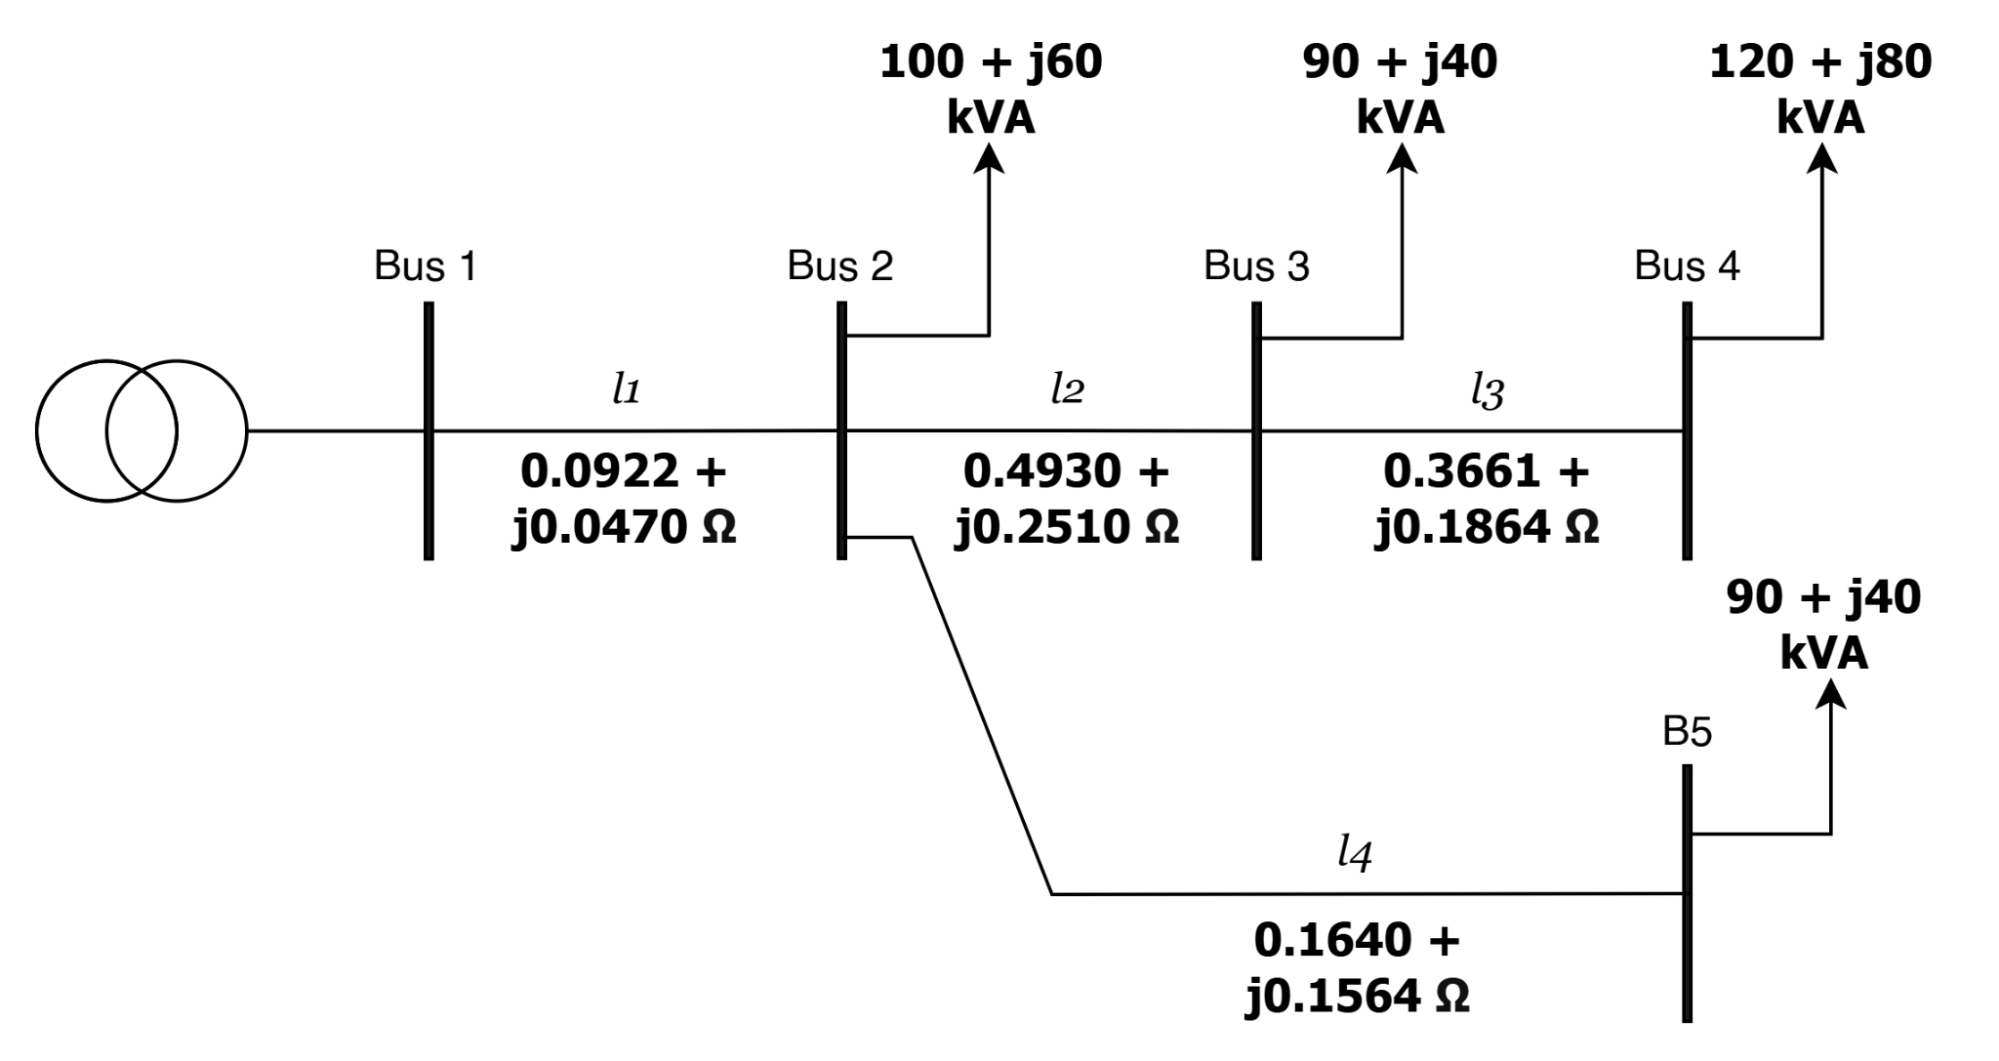
\includegraphics[width=0.4\textwidth]{5buswithdata.png}}
	\caption{5-Bus Radial Distribution System.}
	\vspace{-15pt}
	\label{fig:5buswithdata}
\end{figure}
%\setlength{\intextsep}{0pt}

\subsubsection{IEEE 33-Bus System}
The IEEE 33-bus radial distribution system in Fig.~\ref{fig:33bus} includes a main 18-bus feeder and three lateral feeders, with a total demand of 3.715 MW active and 2.3 MVAr reactive power. The base voltage is 12.66 kV, and the base MVA is 100. This system is widely used in studies, providing several published results for performance comparison.


%\setlength{\intextsep}{0pt}

\subsubsection{Variable Load Demand Data}
Historical load demand data, obtained from \cite{Ausgrid_solar_2023}, includes half-hour active power demand for 300 houses connected to the Australian grid from 1 July 2012 to 30 June 2013.

%\vspace{-5pt}
%\vspace{-5ex}
\subsection{Development of Load Profiles}
Fig.~\ref{fig:loadprofileoverview} illustrates the development of the load profiles. From the annual demand of 300 houses, load profiles of 9 randomly selected houses are aggregated and assigned across 32 load buses. The pre-processed data is averaged over specific periods for daily profiles e.g. in the daily load profile, the load demands are categorized by each hour of the day (hours 1-24) and then averaged per hour. The minimum, median, and maximum system demands for the year generate the low, medium, and peak for the 3-hour load profile. Two hourly variable load profiles were developed for 3- and 24-hour periods, with one peak load profile derived from the 3-hour load profile.





\subsection{Load Flow Analysis}
In the optimal distributed generation allocation (ODGA) problem, optimization techniques explore potential DG sizes and sites, while load flow algorithms evaluate these configurations' fitness based on metrics such as losses and reliability. This study uses the backward/forward sweep (BFS) 

%\vspace{-10pt}
\begin{figure}[htbp]
	\centerline{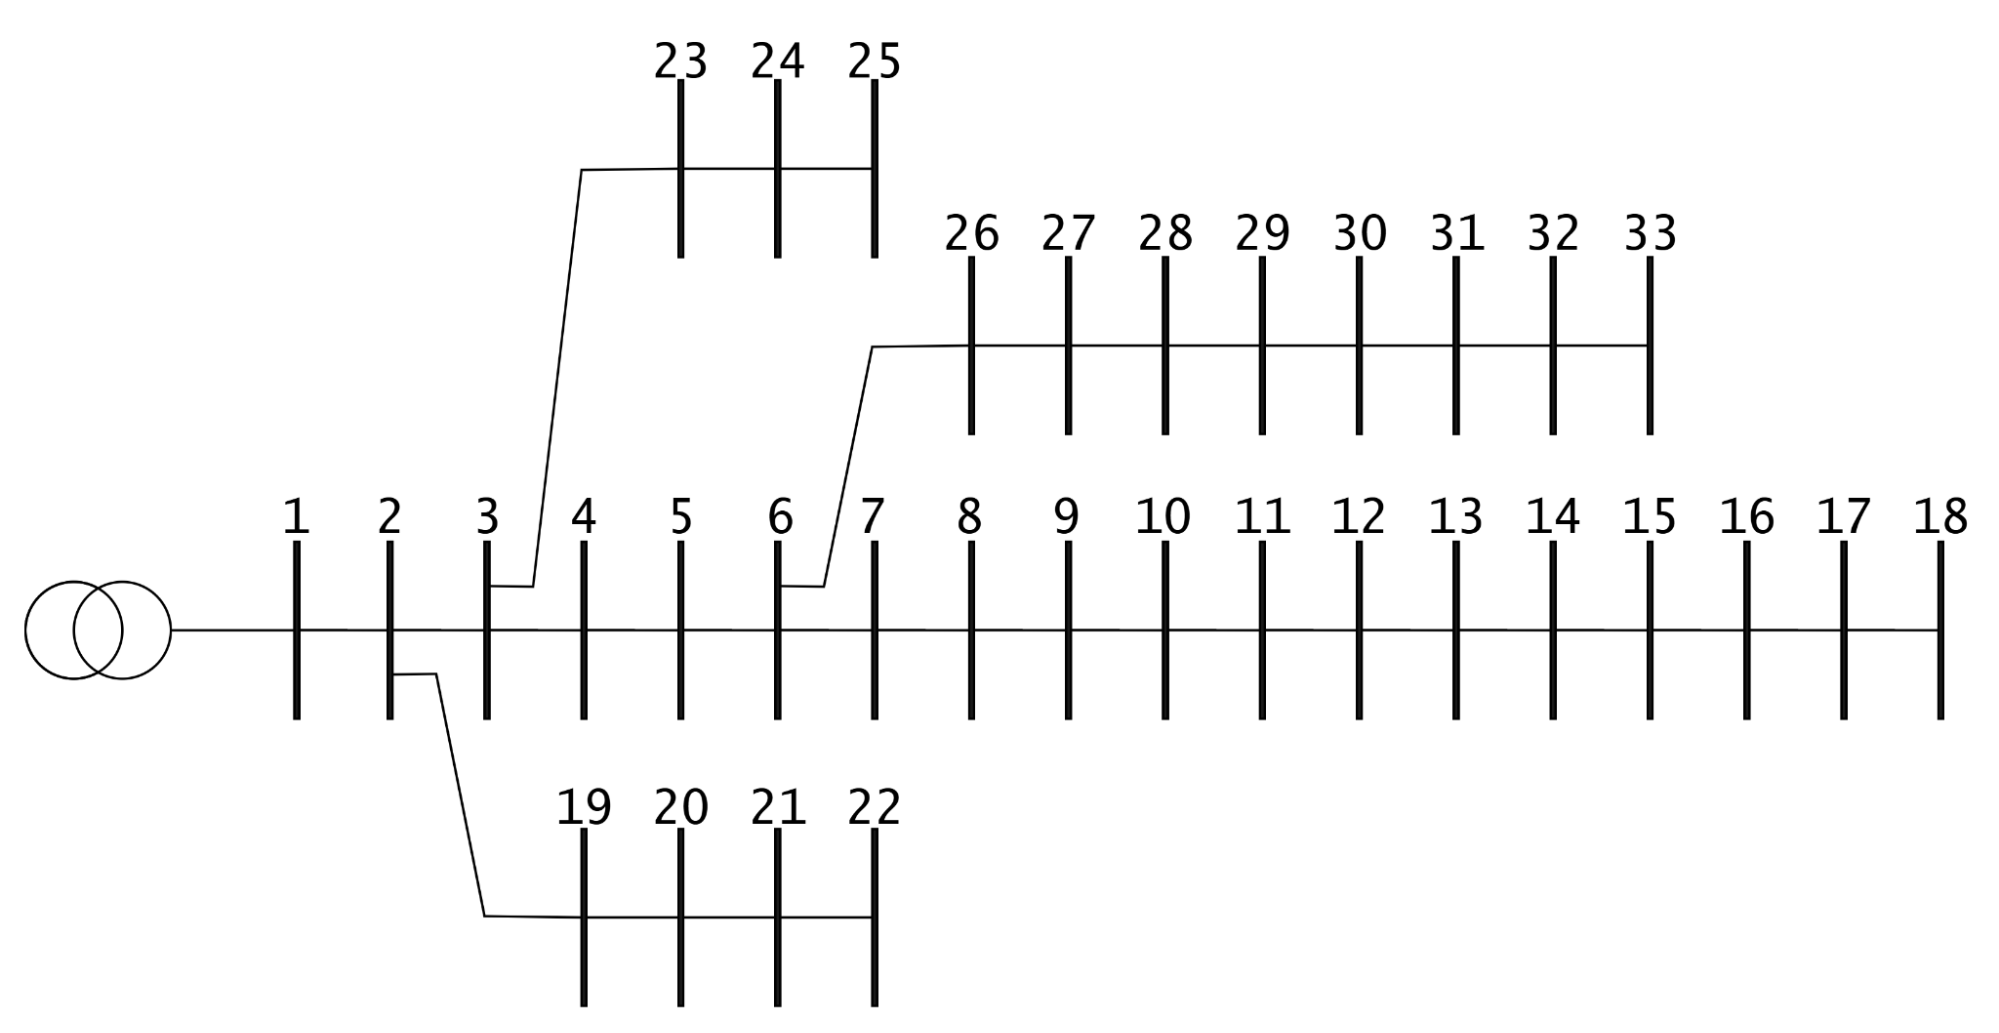
\includegraphics[width=0.45\textwidth]{33bus.png}}
	\caption{IEEE 33-Bus Radial Distribution System.}
	\vspace{-5pt}
	\label{fig:33bus}
\end{figure}

\begin{figure}[htbp]
	\centerline{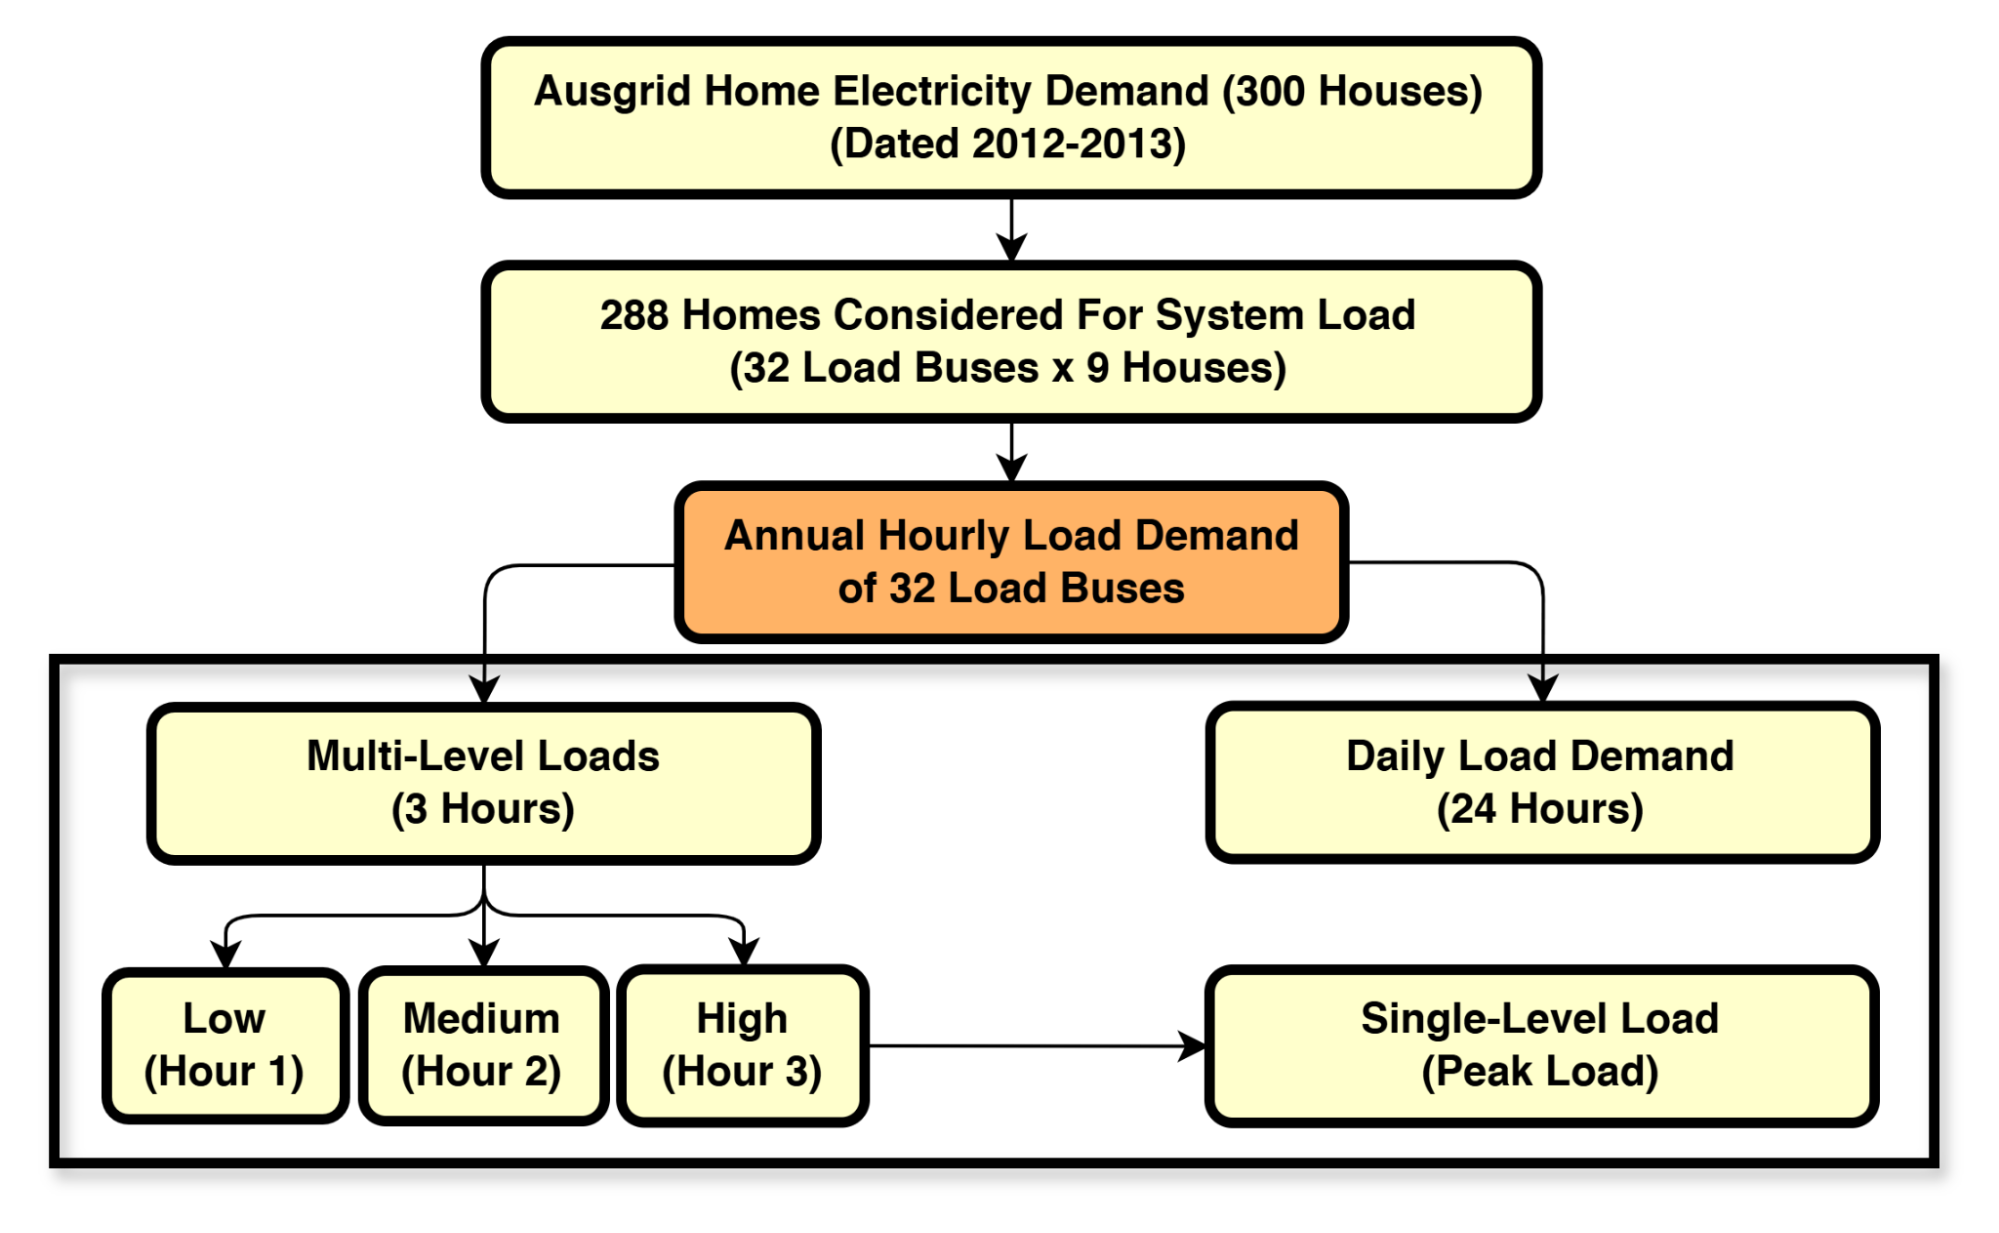
\includegraphics[width=0.43\textwidth]{loadprofileoverview.png}}
	\vspace{-10pt}
	\caption{Load Profile Development Overview.}
	\vspace{-10pt}
	\label{fig:loadprofileoverview}
\end{figure}

\noindent load flow method \cite{BFS}, which has been validated against the results found in \cite{Bouchekara}. 


%\vspace{-1ex}

\subsection{Problem Formulation}
\subsubsection{Objective Function}

\paragraph{Minimization of Power Losses}
For peak load profiles, the objective function minimizes power losses as shown in \eqref{eq:min_powerloss},

\begin{equation}
	PL=\sum_{k=1}^{N_{lines}} \left|I_{k}\right|^{2} \times R_{k}
	\label{eq:min_powerloss}
\end{equation}

where $N_{lines}$ is the total number of lines or branches, $I_k$ is the line current of line $k$, and $R_k$ is the resistance of line $k$.

\paragraph{Minimization of Energy Losses}
For variable loads, the objective function minimizes energy losses as in \eqref{eq:min_energyloss},

\begin{equation}
	EL= \sum_{t=1}^{N_{hours}}  P_{L}^t \Delta t
	\label{eq:min_energyloss}
\end{equation}

where $EL$ represents the energy loss, $P_L^t$ is the active power loss at the time period $t$, and $t$ is the time duration of one hour. $N_{hours}$ is the total number of hours considered in the study, equal to 3 and 24 hours.


\subsubsection{Constraints}
\paragraph{Power Balance}
Equation \eqref{eq:powerbalance} ensures no reverse power flows occur,

\begin{equation}
	P_{S / S}^t+\sum_{i=1}^{N_{D G}} P_{D G}^t=\sum_{i=1}^{N_{\text {Load }}} P_{\text {Load }}^t+\sum_{i=1}^{N_{\text {Line }}} P_{\text {loss }}^t
	\label{eq:powerbalance}
\end{equation}

where $P_{S/S}^t$ is the active power generated by the substation at hour $t$, $P_{DG}^t$ is the active power generated by a DG, $P_{Load}^t$ is the  active power demand, and $P_{Loss}^t$ indicates line losses. 

\paragraph{Voltage}
Post-DG installation bus voltages must fall within the limits in \eqref{eq:voltagemag},

\begin{equation}
	\left|V_{i}^{m i n}\right|\leq\left|V_{i}^{withDG}\right|\leq\left|V_{i}^{m a x}\right|
	\label{eq:voltagemag}
\end{equation}

where \(V_i^{min}\) is $\pm 0.95$ pu and \(V_i^{max}\) is $\pm 1.05$ pu.

\paragraph{Current}
Power lines must not exceed their maximum capacity described in \eqref{eq:currentconst},

\begin{equation}
	I_{i}^{withDG} \leq I_{i}^{max}
	\label{eq:currentconst}
\end{equation}

where \(I_i^{withDG}\) is the current on line \(i\) in the presence of DGs and \(I_i^{max}\) is the maximum current capacity of line \(i\).

\paragraph{Power Generation}
The generated active power of each DG is constrained between the limits in \eqref{eq:const_powergen},

\begin{equation}
	P_{DG}^{min} \leq P_{i}^{DG} \leq P_{DG}^{max} 
	\label{eq:const_powergen}
\end{equation}

where $P_{DGmin}$ is the minimum active power generation limit set to $0$ and $P_{DGmax}$ is the maximum active power generation limit for each DG which is equal to the total active power demand of the system (at hour $i$ for variable loads).

\paragraph{DG Location}
The permissible sites for DG installation are limited by the location of the slack bus (Bus 1) and the total DGs as in \eqref{eq:const_dgloc} and \eqref{eq:const_dgloc2},

\begin{equation}
	2 \leq DG_{loc}\leq N_{Bus}
	\label{eq:const_dgloc}
\end{equation}

\begin{equation}
	DG_1^{\;loc} \ne DG_2^{\;loc} \ne DG_3^{\;loc}
	\label{eq:const_dgloc2}
\end{equation}

where \(DG_{loc}\) represents the potential installation sites for DGs, excluding Bus 1 as it is the slack bus. \(N_{Bus}\) denotes the total number of buses. The second equation ensures that each DG is installed on a different bus, indicated by \(DG_i^{loc}\).

\subsection{Optimization Algorithm Implementation}

Both WOA and E-WOA are continuous optimizers that process continuous variables. Discrete variables are incorporated using the relaxation method during initialization and before fitness evaluation \cite{relaxation}. Algorithm-specific parameters are retained from their original implementations \cite{WOA,EWOA}. Simulations use 200 iterations, a population of 50, and 100 runs. Fig.~\ref{fig:EWOAflowchart} illustrates the flowchart of E-WOA.

\begin{figure}[htbp]
	\centerline{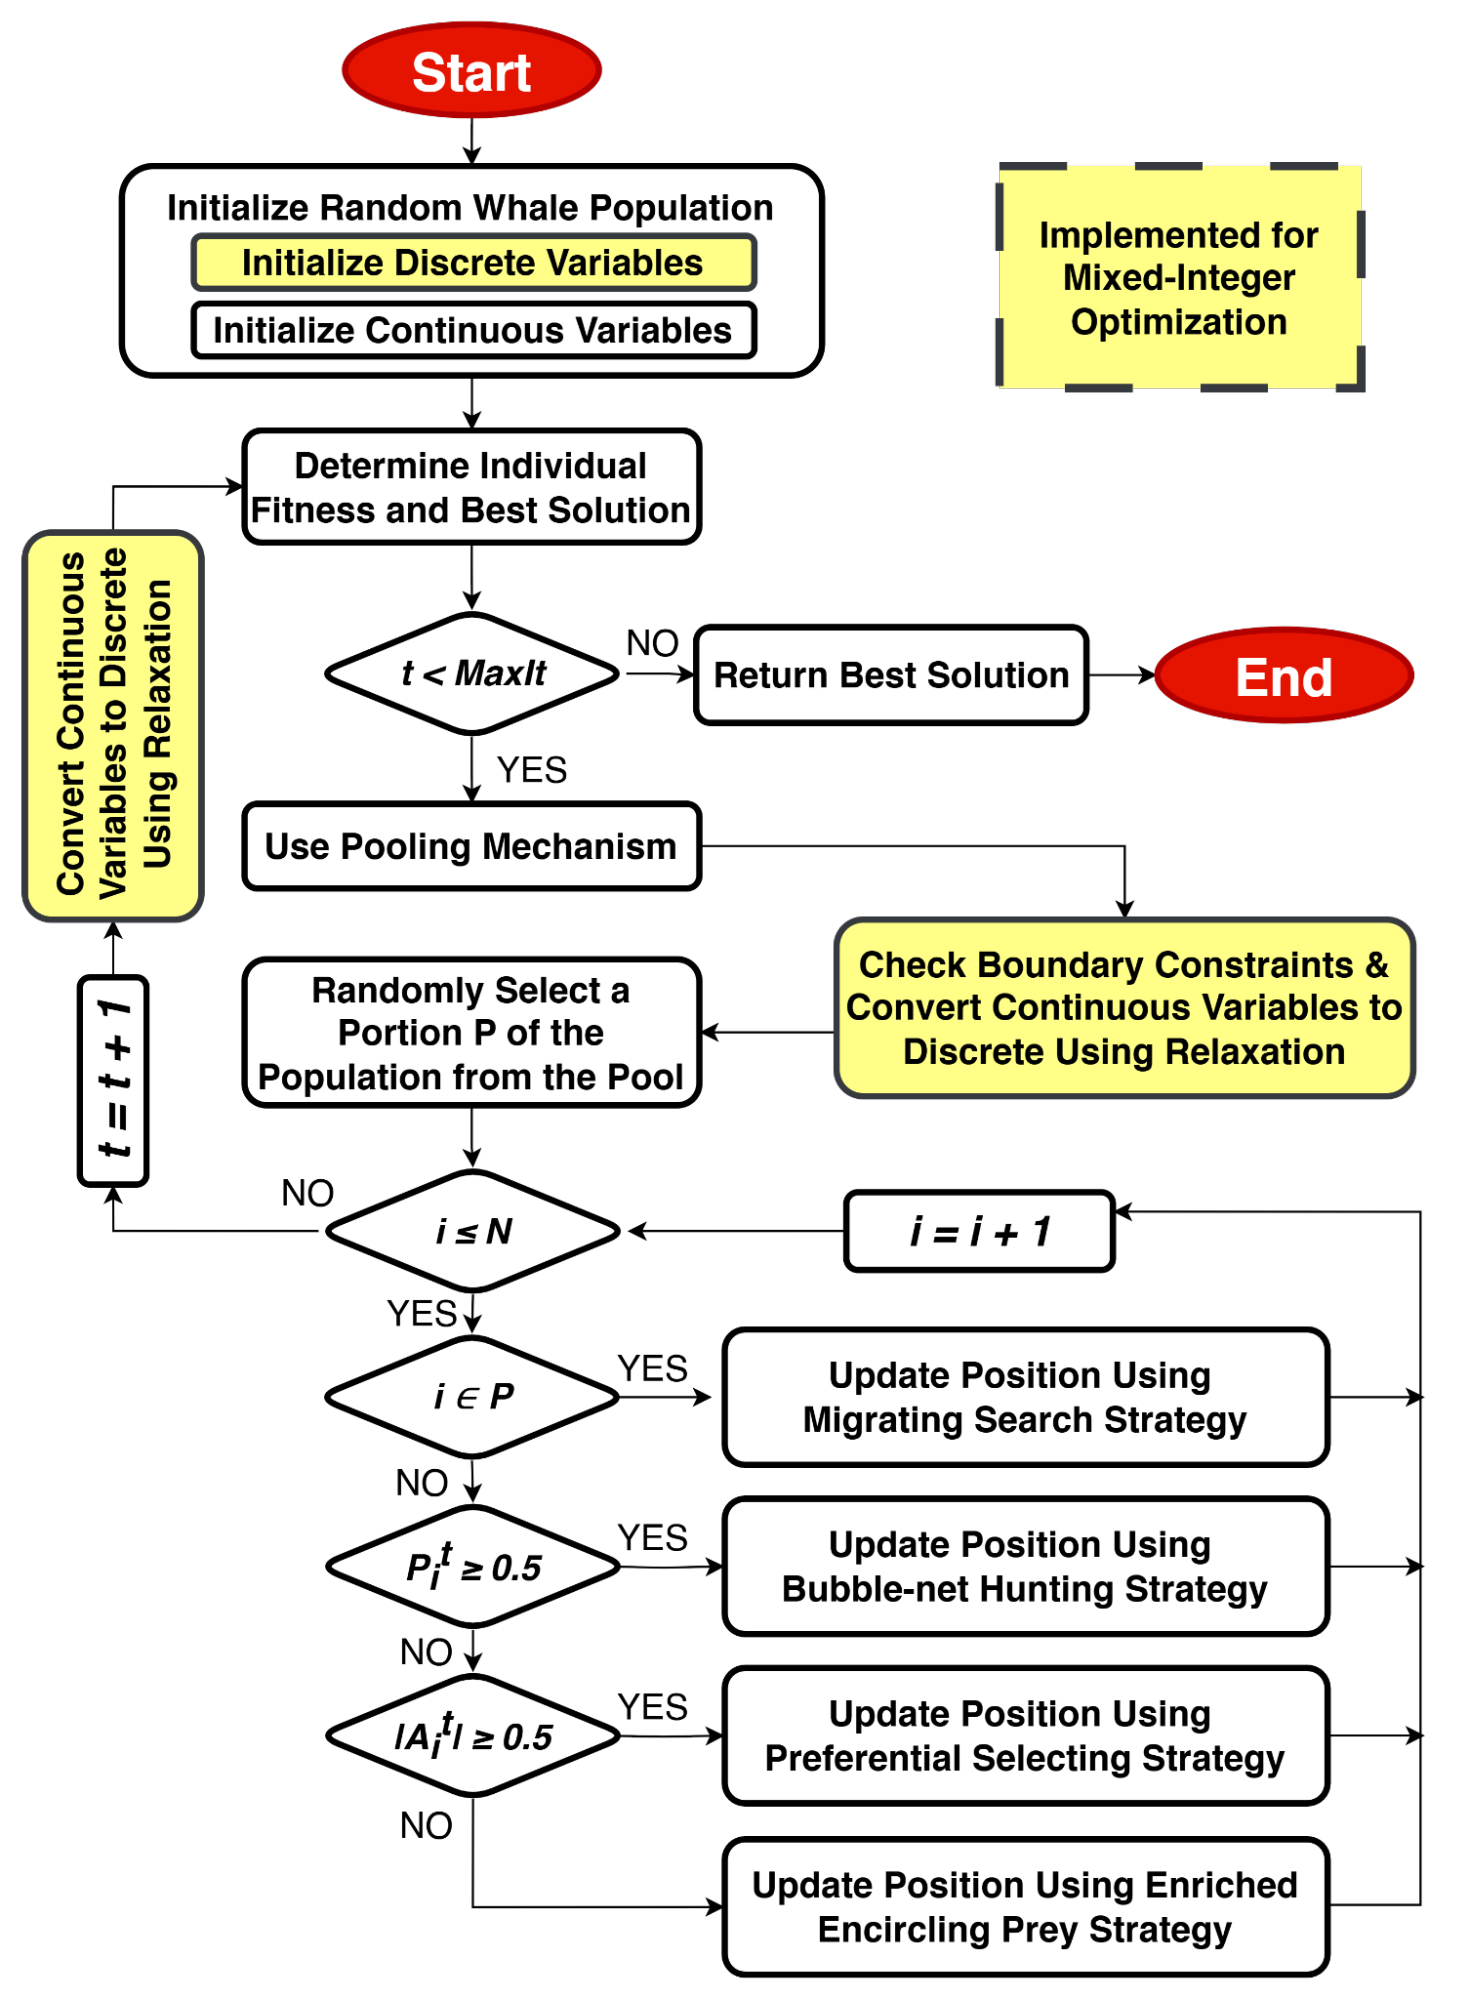
\includegraphics[width=0.42\textwidth]{EWOAflowchart.png}}
	\vspace{-5pt}
	\caption{Enhanced Whale Optimization Algorithm Flowchart.}
	\vspace{-10pt}
	\label{fig:EWOAflowchart}
\end{figure}

\subsection{Test Cases}

Table~\ref{tab:testcases} summarizes the test cases which vary in objective functions, load scenarios, and numbers of DGs.

\begin{table}[htbp]
	\vspace{-10pt}
	\caption{Summary of Test Cases}
	\vspace{-10pt}
	\begin{center}
		\resizebox{\columnwidth}{!}{%
			\begin{tabular}{ccccc}
				\hline
				\textbf{\begin{tabular}[c]{@{}c@{}}Test \\ Case\end{tabular}} &
				\textbf{Obj. Func.} &
				\textbf{Load Profile} &
				\textbf{\begin{tabular}[c]{@{}c@{}}No. of \\ DGs\end{tabular}} &
				\textbf{\begin{tabular}[c]{@{}c@{}}Test \\ System\end{tabular}} \\ \hline
				1 & \begin{tabular}[c]{@{}c@{}}Min. Active Power \\ Loss\end{tabular} & Peak Load (1 Hour)    & Multiple & 33-Bus \\ 
				2 & Min. Energy Loss                                                  & Multi-Level (3 Hours) & Multiple & 33-Bus \\ 
				3 & Min. Energy Loss                                                  & Daily (24 Hours)      & Multiple & 33-Bus \\ 
				 \hline
				A & \begin{tabular}[c]{@{}c@{}}Min. Active Power \\ Loss\end{tabular} &
				\begin{tabular}[c]{@{}c@{}}IEEE 33-Bus Peak Load\\ For Comparison\end{tabular} &
				\begin{tabular}[c]{@{}c@{}}Single/\\ Multiple\end{tabular} &
				33-Bus \\ \hline
			\end{tabular}%
		}
		\label{tab:testcases}
	\end{center}
\end{table}

\vspace{-15pt}
\subsection{Evaluation Metrics}

The results for all test cases are evaluated based on objective function values, number of iterations to converge within 200 iterations, runtime, scalability or average runtime with increasing problem size, and number of violations.

\section{Results and Discussion}\label{sec:results}
The optimal solutions are summarized, and a brief discussion on voltage profiles, and convergence characteristics is provided. The last section compares WOA and E-WOA on a set of evaluation metrics.

\subsection{Comparison with Published Results}

Table~\ref{tab:multipleDGcomparison} details the optimal allocation of three DGs. E-WOA and CBGA-VSA achieve the minimum power loss of 72.785 kW. Although E-WOA attains lower power losses than WOA, WOA still outperforms other recent and improved algorithms.

\subsection{Optimal Solutions for Test Cases}


The optimal DG locations and sizes for Test Cases 1-3 are summarized in Table~\ref{tab:optimalsolutions}. In Case 1, both WOA and E-WOA significantly reduced system losses, with E-WOA achieving slightly lower power loss. As complexity increases in Cases 2-3, E-WOA consistently achieves lower losses than WOA. In Case 3, where the location and dispatch of three DGs were optimized over 24 hours, E-WOA reduced the base energy loss by 89.47\%, compared to WOA's 86.13\%.

\subsection{Voltage Profiles}

Fig.~\ref{fig:voltageprofile} illustrates the voltage profile of the IEEE 33-Bus system for Test Case 3 with increasing loading levels. Both WOA and E-WOA satisfy the voltage constraints of ±5\% deviation from 1 pu while allocating the DGs. Although voltage deviation minimization is not part of the objective function, E-WOA, which achieves lower power losses, also improves the voltage profile more effectively than WOA. Ref. \cite{kashem} notes that minimizing power loss enhances voltage stability, which is related to the improved voltage profile.

\subsection{Convergence Characteristics}

Fig.~\ref{fig:convergencecurve} compares the best convergence curves of the two algorithms for case 3, showing significant differences. WOA converges quickly but prematurely due to limited exploration in later iterations. In contrast, despite encountering infeasible solutions and starting slower, E-WOA continues improving in later iterations, achieving lower objective function values

\begin{table}[htbp]
%	\vspace{-10pt}
	\caption{Optimization Results for Multiple DGs in IEEE 33-Bus System at Unity Power Factor}
	\vspace{-20pt}
	\begin{center}
		\resizebox{\columnwidth}{!}{%
			\begin{tabular}{ccccccc}
				\hline
				\textbf{Year} &
				\textbf{Algorithm} &
				\textbf{\begin{tabular}[c]{@{}c@{}}DG \\ Location\end{tabular}} &
				\multicolumn{3}{c}{\textbf{\begin{tabular}[c]{@{}c@{}}DG Size \\ (kW)\end{tabular}}} &
				\textbf{\begin{tabular}[c]{@{}c@{}}Power \\ Loss (kW)\end{tabular}} \\ \hline
				&
				&
				&
				DG1 &
				DG2 &
				DG3 &
				\\
				\multicolumn{2}{c}{Base} &
				- &
				- &
				- &
				- &
				210.9880 \\
				2016 \cite{HSA_PABC} &
				\begin{tabular}[c]{@{}c@{}}HSA-\\ PABC\end{tabular} &
				14, 24, 30 &
				755.000 &
				1073.000 &
				1068.000 &
				72.8100 \\
				2016 \cite{QOSIMBO} &
				\begin{tabular}[c]{@{}c@{}}QOSIM\\ BO-Q\end{tabular} &
				13, 24, 30 &
				801.600 &
				1090.600 &
				1054.20 &
				72.8000 \\
				2017 \cite{FA} &
				FA &
				13, 17, 31 &
				623.100 &
				261.300 &
				1012.000 &
				87.8300 \\
				2017 \cite{GWO} &
				GWO &
				13, 24, 30 &
				850.020 &
				1103.870 &
				1100.770 &
				73.0600 \\
				2018 \cite{CTLBO} &
				CTLBO &
				13, 24, 30 &
				801.700 &
				1091.300 &
				1053.600 &
				72.7870 \\
				2018 \cite{IMOEHO} &
				IMOEHO &
				14, 24, 30 &
				1057.000 &
				1054.000 &
				1741.000 &
				95.0000 \\
				2019 \cite{MOCDE} &
				MOCDE &
				13, 24, 30 &
				801.840 &
				1091.460 &
				1046.580 &
				72.8480 \\
				2020 \cite{IHHO} &
				HHO &
				14, 24, 30 &
				745.690 &
				1022.690 &
				1135.780 &
				72.9800 \\
				2020 \cite{IHHO} &
				IHHO &
				14, 24, 30 &
				775.540 &
				1080.830 &
				1066.690 &
				72.7900 \\
				\textbf{2020 \cite{CBGAVSA}} &
				\textbf{\begin{tabular}[c]{@{}c@{}}CBGA-\\ VSA\end{tabular}} &
				\textbf{13, 24, 30} &
				\textbf{801.800} &
				\textbf{1091.300} &
				\textbf{1053.600} &
				\textbf{72.7853} \\
				2021 \cite{MRFO} &
				MRFO &
				13, 24, 30 &
				788.276 &
				1017.100 &
				1035.300 &
				72.8760 \\
				\textbf{Present} &
				\textbf{WOA} &
				\textbf{13, 24, 30} &
				\textbf{799.830} &
				\textbf{1047.810} &
				\textbf{1073.150} &
				\textbf{72.8147} \\
				\textbf{Present} &
				\textbf{E-WOA} &
				\textbf{13, 24, 30} &
				\textbf{801.799} &
				\textbf{1091.315} &
				\textbf{1053.601} &
				\textbf{72.7853} \\ \hline
			\end{tabular}%
		}
		\label{tab:multipleDGcomparison}
	\end{center}
\end{table}

%\vspace{-20pt}

\begin{table}[htbp]
	\vspace{-10pt}
	\caption{Best Results for All Test Cases (DGs at 0.9 Power Factor, 200 Iterations, 100 Runs)}
	\vspace{-20pt}
	\begin{center}
		\resizebox{\columnwidth}{!}{%
			\begin{tabular}{ccccccc}
				\hline
				\textbf{Case} &
				\textbf{\begin{tabular}[c]{@{}c@{}}DG \\ Locations\end{tabular}} &
				\multicolumn{3}{c}{\textbf{\begin{tabular}[c]{@{}c@{}}DG Sizes \\ (kW)\end{tabular}}} &
				\textbf{Loss} \\ \hline
				&                                 & DG1                           & DG2                          & DG3                          &                  \\ \cline{3-5}
				Case 1         & \multicolumn{4}{l}{\textit{33-Bus Test System With at Most 3 DGs at Peak Load}}                                                        & kW               \\
				Base           & -                               & -                             & -                            & -                            & 169.389          \\
				WOA            & 6, 15, 30                       & 826.965                       & 785.037                      & 722.887                      & 11.311           \\
				\textbf{E-WOA} & \textbf{6, 15, 30}              & \textbf{807.596}              & \textbf{791.401}             & \textbf{727.083}             & \textbf{11.307}  \\ \hline
				Case 2         & \multicolumn{4}{l}{\begin{tabular}[c]{@{}l@{}}\textit{33-Bus Test System With at Most 3 DGs Across} \\ \textit{3 Loading Levels}\end{tabular}}  & kWh              \\
				Base           & -                               & -                             & -                            & -                            & 216.017          \\
				WOA            & 6, 15, 30                       & 975.723                       & 760.002                      & 628.851                      & 15.479           \\
				\textbf{E-WOA} & \textbf{6, 15, 30}              & \textbf{807.594}              & \textbf{791.402}             & \textbf{727.084}             & \textbf{14.469}  \\ \hline
				Case 3         & \multicolumn{4}{l}{\begin{tabular}[c]{@{}l@{}}\textit{33-Bus Test System With at Most 3 DGs Across} \\ \textit{24 Loading Levels}\end{tabular}} & kWh              \\
				Base           & -                               & -                             & -                            & -                            & 1598.547         \\
				WOA            & 6, 7, 14                        & 914.943                       & 1037.055                     & 933.643                      & 221.838          \\
				\textbf{E-WOA} & \textbf{8, 13, 30}              & \textbf{1094.201}             & \textbf{889.338}             & \textbf{867.780}             & \textbf{168.244} \\ \hline
			\end{tabular}%
		}
		\label{tab:optimalsolutions}
	\end{center}
	\vspace{-10pt}
	
\end{table}
%\vspace{-30pt}

%\noindent E-WOA consistently returned this penalty value across 100 independent runs of 200 iterations each, indicating its failure to identify any solutions that met the required constraints. This shows EWOA's potential limitations in handling highly complex systems. In contrast, WOA successfully identifies solutions, highlighting its robustness despite being less effective in simpler cases.
%\vspace{-15pt}
\newpage
\noindent without premature convergence. This highlights E-WOA's ability to maintain exploration and avoid getting trapped in local optima, although at the cost of slower convergence speed. While this trend is evident in Case 3, in Cases 1, E-WOA converges faster, retaining the same rough staircase pattern compared to WOA's smooth curve.

\begin{figure}[htbp]
%	\vspace{-15pt}
	\centerline{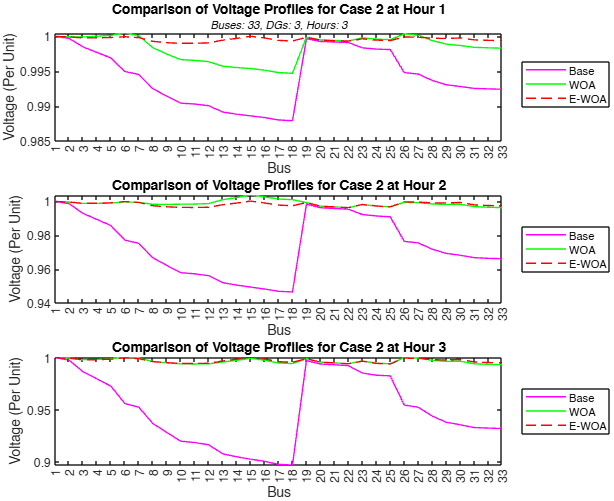
\includegraphics[width=0.9\columnwidth]{voltageprofile.png}}
	\vspace{-5pt}
	\caption{Comparison of Voltage Profiles for Case 2 for Each Hour.}
	\label{fig:voltageprofile}
\end{figure}



\begin{figure}[htbp]
	\centerline{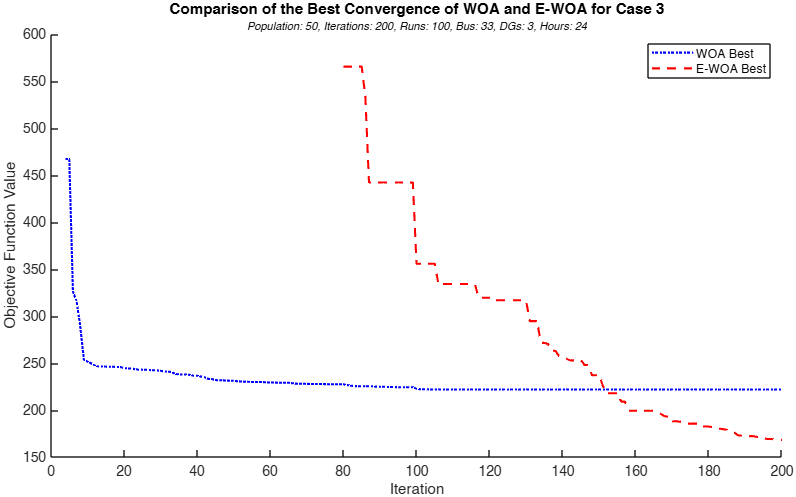
\includegraphics[width=0.46\textwidth]{convergencecurve.png}}
	\vspace{-5pt}
	\caption{Comparison of Best Convergence Curves for Case 3.}
	\vspace{-10pt}
	\label{fig:convergencecurve}
\end{figure}




%\vspace{-10pt}
%\subsection{Convergence Characteristics}
%
%Fig.~\ref{fig:convergencecurve} compares the best convergence curves of the two algorithms for case 4, showing significant differences. WOA converges quickly but prematurely due to limited exploration in later iterations. In contrast, despite encountering infeasible solutions and starting slower, E-WOA continues improving in later iterations, achieving lower objective function values without premature convergence. This highlights E-WOA's ability to maintain exploration and avoid getting trapped in local optima, although at the cost of slower convergence speed. While this trend is evident in Case 4, in Cases 2 and 3, E-WOA converges faster, retaining the same rough staircase pattern compared to WOA's smooth curve, as detailed in the Appendices.

\subsection{Performance Metrics}

\subsubsection{Objective Function Values}
Fig.~\ref{fig:objectivefunction} compares the boxplots of normalized objective function results for both algorithms. E-WOA shows lower variability and median values. Table~\ref{tab:objfunckeyperf} summarizes key performance measures, showing E-WOA's lower mean and standard deviation, suggesting better consistency in finding high-quality solutions in Cases 1-3.

\subsubsection{No. Iterations to Converge}
Fig.~\ref{fig:speedconvergence} compares boxplots of iterations to converge for all cases. For Cases 1-3, WOA's medians are 99, 103, and 113, while E-WOA's are 54, 108, and 199. Although E-WOA converges faster in Case 1, its convergence speed deteriorates in subsequent cases.

\subsubsection{Runtime}
Fig.~\ref{fig:Runtime} compares the boxplots of total runtimes for 200 iterations across 100 runs. In Cases 1-3, WOA has lower median and average runtimes highlighting its computational efficiency.

\subsubsection{No. of Constraint Violations}
Table~\ref{tab:violationsandfeasible} shows that in the small case (Case 1), both WOA and E-WOA consistently find feasible solutions without significant constraint violations. However, in the larger case (Case 3), E-WOA encounters more constraint violations, indicating difficulty in navigating larger search spaces, while WOA maintains a lower violation count. Significantly, WOA found feasible solutions in 42 runs in Case 3, whereas E-WOA found feasible solutions in only 17 runs.

\subsubsection{Scalability}
Table~\ref{tab:scalability} shows a significant increase in average runtimes as the number of variables increases from Case 2 to 3. WOA outperforms E-WOA in average runtime for Cases 1-3 due to its simpler implementation. Previous sections reveal E-WOA's limitations in larger cases, including higher iterations to converge in Cases 2 and 3, higher average runtimes in Cases 2 and 3, and more iterations with constraint violations in Cases 3. These results indicate E-WOA's poor potential in handling large-scale and complex problems, demonstrating inferior scalability compared to the standard WOA.

\section{Conclusion}\label{sec:conclusion}
In this study, the Enhanced Whale Optimization Algorithm (E-WOA) was applied to optimally allocate distributed generation units in the IEEE 33-Bus system, focusing on minimizing power losses and accommodating  load variations through low-mid-peak, and daily load profiles.

%\vspace{-15pt}

\begin{figure}[htbp]
	\vspace{-13pt}
	\centerline{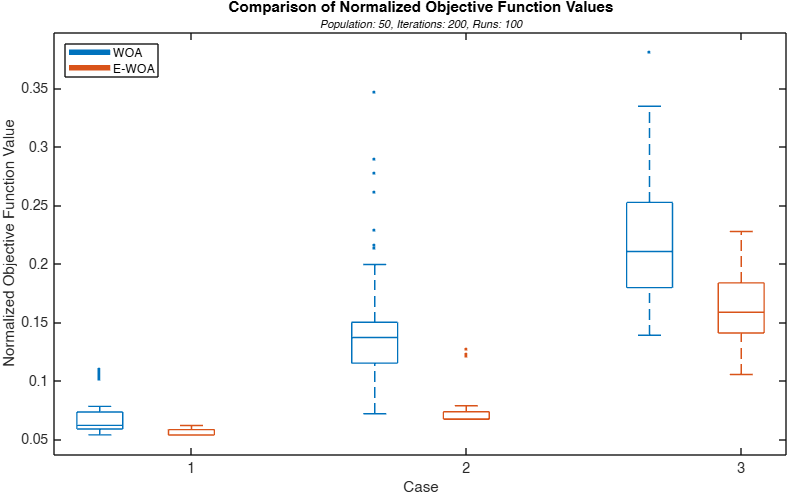
\includegraphics[width=1\columnwidth]{objectivefunction.png}}
	\vspace{-10pt}
	\caption{Box Plot Comparison of the Normalized Objective Function Values Obtained by WOA and E-WOA for Cases 1-3.}
	\vspace{-5pt}
	\label{fig:objectivefunction}
\end{figure}

%\vspace{-15pt}

\begin{figure}[htbp]
	\vspace{-20pt}
	\centerline{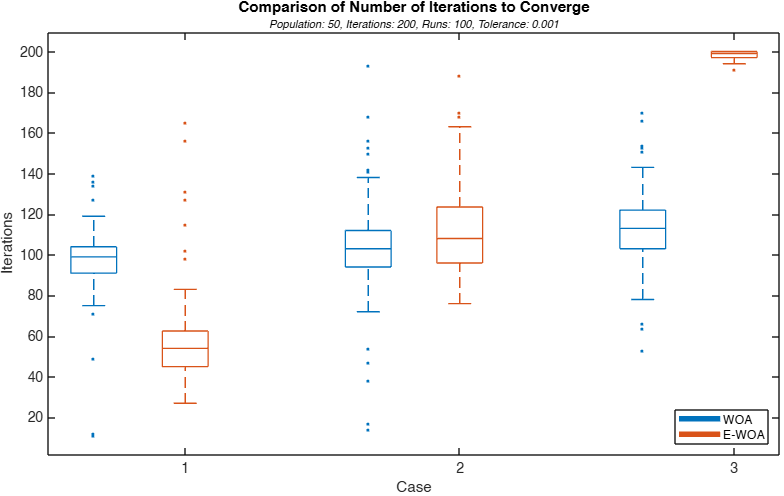
\includegraphics[width=1\columnwidth]{speedconvergence.png}}
	\vspace{-5pt}
	\caption{Box Plot Comparison of Number of Iterations to Converge for 100 Independent Runs.}
	\vspace{-10pt}
	\label{fig:speedconvergence}
\end{figure}

\begin{figure}[htbp]
\vspace{-20pt}
\centerline{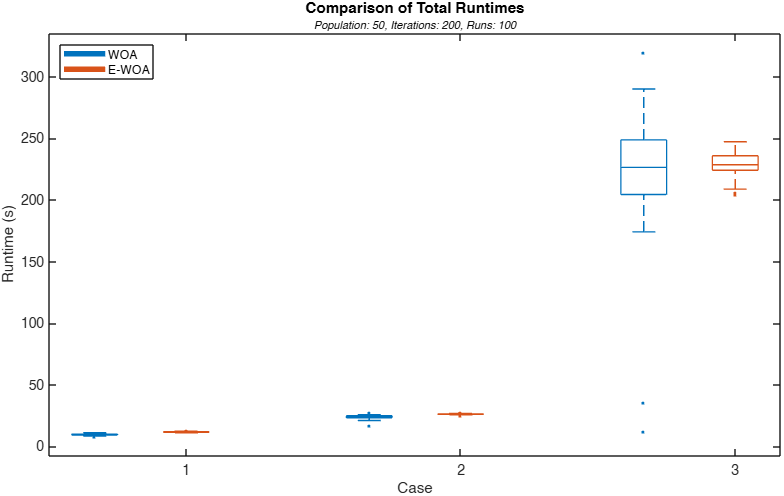
\includegraphics[width=1\columnwidth]{Runtime.png}}
\vspace{-5pt}
\caption{Box Plot Comparison of Total Runtimes.}
\vspace{-10pt}
\label{fig:Runtime}
\end{figure}

\begin{table}[htbp]
	\vspace{-5pt}
	\caption{Comparison of Key Performance Measures of Objective Function Results}
	\vspace{-20pt}
	\begin{center}
		\resizebox{\columnwidth}{!}{%
			\begin{tabular}{ccccccc}
				\hline
				& \multicolumn{2}{c}{\textbf{Mean}} & \multicolumn{2}{c}{\textbf{Standard Deviation}} & \multicolumn{2}{c}{\textbf{Minimum}} \\ \cline{2-7} 
				& \textbf{\textit{WOA}}   & \textbf{\textit{E-WOA}}   & \textbf{\textit{WOA}}          & \textbf{\textit{E-WOA}}          & \textbf{\textit{WOA}}     & \textbf{\textit{E-WOA}}    \\ \hline
				Case 1 & 14.6446  & 11.7118  & 2.5773   & 1.0800   & 11.3111  & 11.3073  \\
				Case 2 & 30.5655  & 16.2833  & 5.9251   & 3.7039   & 15.4794  & 14.4691  \\
				Case 3 & 349.2446 & 257.4618 & 146.3024 & 32.8077  & 221.8375 & 168.2436 \\\hline
			\end{tabular}%
		}
		\label{tab:objfunckeyperf}
	\end{center}
\end{table}








%Results indicate that E-WOA is effective, often outperforming other advanced algorithms in smaller-scale ODGA problems through its improved search strategies and population diversity. However, E-WOA struggles with larger, more complex problems due to longer runtimes, slower convergence, and scalability issues, which diminish its advantages over the standard Whale Optimization Algorithm (WOA).
%\newpage



%\newline

%\begin{table}[htbp]
%	\vspace{-5pt}
%	\caption{Iterations With Violations and Runs With Feasible Solutions}
%	\vspace{-15pt}
%	\begin{center}
%		\resizebox{\columnwidth}{!}{%
%			\begin{tabular}{ccccccc}
%				\hline
%				\multirow{2}{*}{\textbf{Algorithm}} & \multirow{2}{*}{\textbf{Criteria}} & \multicolumn{5}{c}{\textbf{Case 1}} \\ \cline{3-7} 
%				&            & \textit{1}   & \textit{2}          & \textit{3}            & \textit{4}              & \textit{5}              \\ \hline
%				\multirow{2}{*}{WOA}   & I.w.V.$^{\mathrm{a}}$    & 0   & 8          & 745          & \textbf{13340} & \textbf{17453} \\
%				& R.w.F.S.$^{\mathrm{b}}$  & 100 & 100        & 99           & \textbf{42}    & \textbf{16}    \\ \hline
%				\multirow{2}{*}{E-WOA} & I.w.V. & 0   & \textbf{0} & \textbf{1}   & 17765          & 20000          \\
%				& R.w.F.S.   & 100 & 100        & \textbf{100} & 17             & 0              \\ \hline
%				\multicolumn{7}{l}{$^{\mathrm{a}}${\scriptsize I.w.V. is Iterations with Violations.}} \\
%				\multicolumn{7}{l}{$^{\mathrm{b}}${\scriptsize R.w.F.S. is Runs with Feasible Solutions.}} \\
%			\end{tabular}%
%		}
%		\label{tab:violationsandfeasible}
%	\end{center}
%\end{table}


\begin{table}[htbp]
%	\vspace{-5pt}
	\caption{Iterations With Violations and Runs With Feasible Solutions}
	\tiny
	\vspace{-15pt}
	\begin{center}
		\resizebox{\columnwidth}{!}{%
			\begin{tabular}{ccccc}
				\hline
				\multirow{2}{*}{\textbf{Algorithm}} & \multirow{2}{*}{\textbf{Criteria}} & \multicolumn{3}{c}{\textbf{Cases}} \\ \cline{3-5} 
				&      & \textit{1}          & \textit{2}            & \textit{3}                 \\ \hline
				\multirow{2}{*}{WOA}   & I.w.V.$^{\mathrm{a}}$    &  8          & 745          & \textbf{13340}  \\
				& R.w.F.S.$^{\mathrm{b}}$   & 100        & 99           & \textbf{42}   \\ \hline
				\multirow{2}{*}{E-WOA} & I.w.V.    & \textbf{0} & \textbf{1}   & 17765                   \\
				& R.w.F.S.  & 100        & \textbf{100} & 17               \\ \hline
				\multicolumn{5}{l}{$^{\mathrm{a}}${\tiny I.w.V. is Iterations with Violations.}} \\
				\multicolumn{5}{l}{$^{\mathrm{b}}${\tiny R.w.F.S. is Runs with Feasible Solutions.}} \\
			\end{tabular}%
		}
		\label{tab:violationsandfeasible}
	\end{center}
\end{table}


\begin{table}[htbp]
%	\vspace{-5pt}
	\centering
	\vspace{-10pt}
	\caption{Average Total Runtimes for Each Case}
	\vspace{-5pt}
	\label{tab:scalability}
	\tiny
	\resizebox{\columnwidth}{!}{%
		\begin{tabular}{ccccc}
			\hline
			&  & \textbf{Case 1} & \textbf{Case 2} & \textbf{Case 3} \\ \hline
			\multirow{2}{*}{\begin{tabular}[c]{@{}c@{}}Case Specs.\\ (33-Bus)\end{tabular}} & DGs & 3 & 3 & 3 \\
			& Hours & 1 & 3 & 24 \\ \hline
			\multirow{3}{*}{Variables} & Locations & 3 & 3 & 3 \\
			& \begin{tabular}[c]{@{}c@{}}Size/\\ Dispatch$^{\mathrm{a}}$\end{tabular} & 3 & 9 & 72 \\
			& Total & \textbf{6} & \textbf{12} & \textbf{75} \\ \hline
			\multirow{2}{*}{\begin{tabular}[c]{@{}c@{}}Mean\\ (s)\end{tabular}} & WOA & \textbf{9.51} & \textbf{23.949} & \textbf{223.80} \\
			& E-WOA & 11.61 & 26.11 & 228.66 \\ \hline
			\multicolumn{5}{l}{$^{\mathrm{a}}${Dispatch = (No. of DGs) * (No. of Hours).}} \\
		\end{tabular}%
	}
	\vspace{-5pt}
\end{table}

The results demonstrate that both WOA and E-WOA are effective in solving the ODGA problem, with E-WOA performing on par with or better than recent improved and hybrid optimization algorithms in finding the global optimum. An in-depth comparison reveals the impact of E-WOA's improved search strategies and population diversity. These enable E-WOA to consistently find high-quality solutions for problems with few variables. However, these enhancements lead to longer runtimes, slower convergence for large problems, worse constraint handling, and poor scalability, failing to consistently find feasible solutions in large-scale problems. While E-WOA outperforms WOA in smaller cases, its advantages diminish as problem complexity increases.

Future research should aim to refine E-WOA for large-scale applications, explore its performance across different electrical system configurations, and incorporate modern load demands and renewable generation profiles to enhance the simulation's practicality and relevance.



\begin{thebibliography}{00}
%	\vspace{-5pt}

\bibitem{IEA} IEA, “Renewables - energy system,” IEA, 2023. https://www.iea.org/energy-system/renewables

\bibitem{WOAreview2} T. Yuvaraj, K. R. Devabalaji, and S. B. Thanikanti, “Simultaneous allocation of dg and dstatcom using whale optimization algorithm,” Iranian Journal of Science and Technology, Transactions of Electrical Engineering, vol. 44, no. 2, pp. 879–896, Sep. 2019, doi: https://doi.org/10.1007/s40998-019-00272-w.

\bibitem{Levy Flight} H. Chen, Y. Xu, M. Wang, and X. Zhao, “A balanced whale optimization algorithm for constrained engineering design problems,” Appl. Math. Model., vol. 71, pp. 45–59, Jul. 2019, doi: 10.1016/j.apm.2019.02.004.

\bibitem{Adaptive} 	W. Guo, T. Liu, F. Dai, and P. Xu, “An improved whale optimization algorithm for forecasting water resources demand,” Appl. Soft Comput., vol. 86, p. 105925, Jan. 2020, doi: 10.1016/j.asoc.2019.105925.

\bibitem{WOAreview} M. H. Nadimi-Shahraki, H. Zamani, Zahra Asghari Varzaneh, and Seyedali Mirjalili, “A systematic review of the whale optimization algorithm: theoretical foundation, improvements, and hybridizations,” Archives of Computational Methods in Engineering, May 2023, doi: https://doi.org/10.1007/s11831-023-09928-7.

\bibitem{EWOA} M. H. Nadimi-Shahraki, H. Zamani, and S. Mirjalili, “Enhanced whale optimization algorithm for medical feature selection: A COVID-19 case study,” Comput. Biol. Med., vol. 148, p. 105858, Sep. 2022, doi: 10.1016/j.compbiomed.2022.105858.

\bibitem{purluseasonal} M. Purlu and B. E. Turkay, “Optimal allocation of renewable distributed generations using heuristic methods to minimize annual energy losses and voltage deviation index,” IEEE Access, vol. 10, pp. 21455–21474, 2022, doi: https://doi.org/10.1109/access.2022.3153042.



\bibitem{Ausgrid_solar_2023}
Ausgrid, ``Solar Home Electricity Data,''
\url{https://www.ausgrid.com.au/Industry/Our-Research/Data-to-share/Solar-home-electricity-data}, 2023. [Online; accessed 16-October-2023].

\bibitem{BFS} W. H. Kersting, Distribution System Modeling and Analysis, 4th ed. Boca Raton: CRC Press, 2017. doi: 10.1201/9781315120782.

\bibitem{Bouchekara} H. R. E.-H. Bouchekara, Y. Latreche, K. Naidu, H. Mokhlis, W. M. Dahalan, and M. S. Javaid, “Comprehensive review of radial distribution test systems for power system distribution education and research,” Resource-Efficient Technologies, 2019.

\bibitem{relaxation} F. Wang, H. Zhang, and A. Zhou, “A particle swarm optimization algorithm for mixed-variable optimization problems,” Swarm Evol. Comput., vol. 60, p. 100808, Feb. 2021, doi: 10.1016/j.swevo.2020.100808.

\bibitem{WOA} S. Mirjalili and A. Lewis, “The whale optimization algorithm,” Adv. Eng. Softw., vol. 95, pp. 51–67, May 2016, doi: 10.1016/j.advengsoft.2016.01.008.

\bibitem{HSA_PABC} K. Muthukumar and S. Jayalalitha, “Optimal placement and sizing of distributed generators and shunt capacitors for power loss minimization in radial distribution networks using hybrid heuristic search optimization technique,” Int. J. Electr. Power Energy Syst., vol. 78, pp. 299–319, Jun. 2016, doi: 10.1016/j.ijepes.2015.11.019.

\bibitem{QOSIMBO} S. Sharma, S. Bhattacharjee, and A. Bhattacharya, “Quasi-oppositional swine influenza model based optimization with quarantine for optimal allocation of dg in radial distribution network,” Int. J. Electr. Power Energy Syst., vol. 74, pp. 348–373, Jan. 2016, doi: 10.1016/j.ijepes.2015.07.034.

\bibitem{FA} S. Sudabattula and M. Kowsalya, “Optimal allocation of multiple distributed generators in distribution system using firefly algorithm,” J. Electr. Eng., vol. 17, pp. 1–12, Jan. 2017, doi: 10.23751/pn.v19i1.5386.

\bibitem{GWO} A.-R. S. El-Sayed, “Optimal Number Size and Location of Distributed Generation Units in Radial Distribution Systems Using Grey Wolf Optimizer.” Accessed: Apr. 28, 2024. [Online]. Available: \url{https://www.researchgate.net/publication/313841863_Optimal_Number_Size_and_Location_of_Distributed_Generation_Units_in_Radial_Distribution_Systems_Using_Grey_Wolf_Optimizer}

\bibitem{CTLBO} I. A. Quadri, S. Bhowmick, and D. Joshi, “A comprehensive technique for optimal allocation of distributed energy resources in radial distribution systems,” Appl. Energy, vol. 211, pp. 1245–1260, Feb. 2018, doi: 10.1016/j.apenergy.2017.11.108.

\bibitem{IMOEHO} N. K. Meena, S. Parashar, A. Swarnkar, N. Gupta, and K. R. Niazi, “Improved elephant herding optimization for multiobjective DER accommodation in distribution systems,” IEEE Trans. Ind. Inform., vol. 14, no. 3, pp. 1029–1039, Mar. 2018, doi: 10.1109/TII.2017.2748220.

\bibitem{MOCDE} S. Kumar, K. K. Mandal, and N. Chakraborty, “Optimal dg placement by multi-objective opposition based chaotic differential evolution for techno-economic analysis,” Appl. Soft Comput., vol. 78, pp. 70–83, May 2019, doi: 10.1016/j.asoc.2019.02.013.

\bibitem{IHHO} A. Selim, S. Kamel, A. S. Alghamdi, and F. Jurado, “Optimal placement of dgs in distribution system using an improved harris hawks optimizer based on single- and multi-objective approaches,” IEEE Access, vol. 8, pp. 52815–52829, 2020, doi: 10.1109/ACCESS.2020.2980245.

\bibitem{CBGAVSA} O. D. Montoya, W. Gil-González, and C. Orozco-Henao, “Vortex search and chu-beasley genetic algorithms for optimal location and sizing of distributed generators in distribution networks: a novel hybrid approach,” Engineering Science and Technology, an International Journal, vol. 23, no. 6, pp. 1351–1363, Dec. 2020, doi: https://doi.org/10.1016/j.jestch.2020.08.002.

\bibitem{MRFO} M. G. Hemeida, A. A. Ibrahim, A.-A. A. Mohamed, S. Alkhalaf, and A. M. B. El-Dine, “Optimal allocation of distributed generators dg based manta ray foraging optimization algorithm (MRFO),” Ain Shams Eng. J., vol. 12, no. 1, pp. 609–619, Mar. 2021, doi: 10.1016/j.asej.2020.07.009.

\bibitem{kashem} M. A. Kashem and M. Moghavvemi, “Maximizing radial voltage stability and load balancing via loss minimization in distribution networks,” in Proceedings of EMPD ’98. 1998 International Conference on Energy Management and Power Delivery (Cat. No.98EX137), Mar. 1998, pp. 91–96 vol.1. doi: 10.1109/EMPD.1998.705437.


\end{thebibliography}

%\newpage
%\section*{Appendices}
%
%\subsection{System Data}
%This section details the bus and line data used in the study.
%
%\subsubsection{5-Bus Test System}
%The total active power demand of this distribution system is 400 kW.
%
%\begin{table}[htbp]
%	\centering
%	\caption{Bus and Line Data of a 5-Bus RDS}
%	\resizebox{\columnwidth}{!}{%
%	\begin{tabular}{|cccccccc|}
%		\hline
%		\multicolumn{1}{|c|}{\multirow{2}*{\centering \begin{tabular}[c]{@{}c@{}}Line\\ No.\end{tabular}}} & 
%		\multicolumn{1}{c|}{\multirow{2}{*}{\begin{tabular}[c]{@{}c@{}}Snd.\\ Bus\end{tabular}}} & 
%		\multicolumn{1}{c|}{\multirow{2}{*}{\begin{tabular}[c]{@{}c@{}}Rcv. Bus\\ (Bus No.)\end{tabular}}} & \multicolumn{2}{c|}{Load at Rcv. Bus} & \multicolumn{2}{c|}{Line Impedance} & \multirow{2}*{\centering \begin{tabular}[c]{@{}c@{}}Imax\\ (Amps)\end{tabular}} \\ \cline{4-7}
%		
%		\multicolumn{1}{|c|}{} & \multicolumn{1}{c|}{} & \multicolumn{1}{c|}{} & \multicolumn{1}{c|}{P (kW)} & \multicolumn{1}{c|}{Q (kVAr)} & \multicolumn{1}{c|}{R (ohms)} & \multicolumn{1}{c|}{X (ohms)} &  \\ \hline
%		\multicolumn{1}{|c|}{} & \multicolumn{1}{c|}{S/S} & \multicolumn{1}{c|}{1} & \multicolumn{1}{c|}{0} & \multicolumn{1}{c|}{0} & \multicolumn{1}{c|}{0} & \multicolumn{1}{c|}{0} & N/A \\ \hline
%		\multicolumn{1}{|c|}{1} & \multicolumn{1}{c|}{1} & \multicolumn{1}{c|}{2} & \multicolumn{1}{c|}{100} & \multicolumn{1}{c|}{60} & \multicolumn{1}{c|}{0.0922} & \multicolumn{1}{c|}{0.0470} & 400 \\ \hline
%		\multicolumn{1}{|c|}{2} & \multicolumn{1}{c|}{2} & \multicolumn{1}{c|}{3} & \multicolumn{1}{c|}{90} & \multicolumn{1}{c|}{40} & \multicolumn{1}{c|}{0.4930} & \multicolumn{1}{c|}{0.2510} & 400 \\ \hline
%		\multicolumn{1}{|c|}{3} & \multicolumn{1}{c|}{3} & \multicolumn{1}{c|}{4} & \multicolumn{1}{c|}{120} & \multicolumn{1}{c|}{80} & \multicolumn{1}{c|}{0.3661} & \multicolumn{1}{c|}{0.1864} & 400 \\ \hline
%		\multicolumn{1}{|c|}{4} & \multicolumn{1}{c|}{2} & \multicolumn{1}{c|}{5} & \multicolumn{1}{c|}{90} & \multicolumn{1}{c|}{40} & \multicolumn{1}{c|}{0.1640} & \multicolumn{1}{c|}{0.1564} & 400 \\ \hline
%		\multicolumn{4}{|c|}{Base MVA: 100 MVA} & \multicolumn{4}{c|}{Base Voltage: 12.66 kV} \\ \hline
%	\end{tabular}%
%	}
%	\label{tab:buslinedata5bus}
%\end{table}
%
%Table~\ref{tab:loadflowresult} compares the load flow results of the implemented BFS with published results. Running BFS on the 33-Bus yields solutions consistent with the published results in \cite{Bouchekara} .
%
%
%\begin{table}[htbp]
%	\caption{Summary of IEEE 33-Bus Load Flow Analysis Results}
%	\begin{center}
%		\begin{tabular}{ccc}
%			\hline
%			\textbf{IEEE 33-Bus Test System} & \textbf{BFS} & \textbf{Bouchekara et al. \cite{Bouchekara}} \\ \hline
%			Tot. Active Power Loss (kW)      & 202.6771     & 202.6771                   \\
%			Tot. Reactive Power Loss (kVAr)  & 135.1410     & 135.1410                   \\
%			Minimum Voltage (pu)             & 0.913        & 0.913                      \\
%			Min. Voltage Bus Location        & Bus 18       & Bus 18                     \\	\hline
%		\end{tabular}
%		\label{tab:loadflowresult}
%	\end{center}
%\end{table}
%
%\subsubsection{IEEE 33-Bus System}
%The total demand is 3.715 MW active and 2.3 MVAr reactive power. Table \ref{tab:33busdata} summarizes the bus and line data.
%
%\begin{table}[htbp]
%	\centering
%	\caption{Bus and Line Data of the IEEE33-Bus RDS}
%	\label{tab:33busdata}
%	\resizebox{\columnwidth}{!}{%
%		\begin{tabular}{|ccccccccc|}
%			\hline
%			\multicolumn{1}{|c|}{\multirow{2}{*}{\textbf{\begin{tabular}[c]{@{}c@{}}Line \\ No.\end{tabular}}}} &
%			\multicolumn{1}{c|}{\multirow{2}{*}{\textbf{\begin{tabular}[c]{@{}c@{}}Snd.\\ Bus\end{tabular}}}} &
%			\multicolumn{1}{c|}{\multirow{2}{*}{\textbf{\begin{tabular}[c]{@{}c@{}}Rcv.\\ Bus\\ (Bus \\ no.)\end{tabular}}}} &
%			\multicolumn{3}{c|}{\textbf{Load at Rcv. Bus}} &
%			\multicolumn{2}{c|}{\textbf{\begin{tabular}[c]{@{}c@{}}Line \\ Impedance\end{tabular}}} &
%			\multirow{2}{*}{\textbf{Imax}} \\ \cline{4-8}
%			\multicolumn{1}{|c|}{} &
%			\multicolumn{1}{c|}{} &
%			\multicolumn{1}{c|}{} &
%			\multicolumn{1}{c|}{\textbf{\begin{tabular}[c]{@{}c@{}}P\\ (kW)\end{tabular}}} &
%			\multicolumn{1}{c|}{\textbf{\begin{tabular}[c]{@{}c@{}}Q\\ (kVAr)\end{tabular}}} &
%			\multicolumn{1}{c|}{\textbf{Pf}} &
%			\multicolumn{1}{c|}{\textbf{\begin{tabular}[c]{@{}c@{}}R \\ (ohms)\end{tabular}}} &
%			\multicolumn{1}{c|}{\textbf{\begin{tabular}[c]{@{}c@{}}X \\ (ohms)\end{tabular}}} &
%			\\ \hline
%			\multicolumn{1}{|c|}{} &
%			\multicolumn{1}{c|}{S/S} &
%			\multicolumn{1}{c|}{1} &
%			\multicolumn{1}{c|}{0} &
%			\multicolumn{1}{c|}{0} &
%			\multicolumn{1}{c|}{0} &
%			\multicolumn{1}{c|}{0} &
%			\multicolumn{1}{c|}{0} &
%			N/A \\ \hline
%			\multicolumn{1}{|c|}{1} &
%			\multicolumn{1}{c|}{1} &
%			\multicolumn{1}{c|}{2} &
%			\multicolumn{1}{c|}{100} &
%			\multicolumn{1}{c|}{60} &
%			\multicolumn{1}{c|}{0.8575} &
%			\multicolumn{1}{c|}{0.0922} &
%			\multicolumn{1}{c|}{0.0470} &
%			400 \\ \hline
%			\multicolumn{1}{|c|}{2} &
%			\multicolumn{1}{c|}{2} &
%			\multicolumn{1}{c|}{3} &
%			\multicolumn{1}{c|}{90} &
%			\multicolumn{1}{c|}{40} &
%			\multicolumn{1}{c|}{0.9138} &
%			\multicolumn{1}{c|}{0.4930} &
%			\multicolumn{1}{c|}{0.2510} &
%			400 \\ \hline
%			\multicolumn{1}{|c|}{3} &
%			\multicolumn{1}{c|}{3} &
%			\multicolumn{1}{c|}{4} &
%			\multicolumn{1}{c|}{120} &
%			\multicolumn{1}{c|}{80} &
%			\multicolumn{1}{c|}{0.8321} &
%			\multicolumn{1}{c|}{0.3661} &
%			\multicolumn{1}{c|}{0.1864} &
%			400 \\ \hline
%			\multicolumn{1}{|c|}{4} &
%			\multicolumn{1}{c|}{4} &
%			\multicolumn{1}{c|}{5} &
%			\multicolumn{1}{c|}{60} &
%			\multicolumn{1}{c|}{30} &
%			\multicolumn{1}{c|}{0.8944} &
%			\multicolumn{1}{c|}{0.3811} &
%			\multicolumn{1}{c|}{0.1941} &
%			400 \\ \hline
%			\multicolumn{1}{|c|}{5} &
%			\multicolumn{1}{c|}{5} &
%			\multicolumn{1}{c|}{6} &
%			\multicolumn{1}{c|}{60} &
%			\multicolumn{1}{c|}{20} &
%			\multicolumn{1}{c|}{0.9487} &
%			\multicolumn{1}{c|}{0.8190} &
%			\multicolumn{1}{c|}{0.7070} &
%			400 \\ \hline
%			\multicolumn{1}{|c|}{6} &
%			\multicolumn{1}{c|}{6} &
%			\multicolumn{1}{c|}{7} &
%			\multicolumn{1}{c|}{200} &
%			\multicolumn{1}{c|}{100} &
%			\multicolumn{1}{c|}{0.8944} &
%			\multicolumn{1}{c|}{0.1872} &
%			\multicolumn{1}{c|}{0.6188} &
%			300 \\ \hline
%			\multicolumn{1}{|c|}{7} &
%			\multicolumn{1}{c|}{7} &
%			\multicolumn{1}{c|}{8} &
%			\multicolumn{1}{c|}{200} &
%			\multicolumn{1}{c|}{100} &
%			\multicolumn{1}{c|}{0.8944} &
%			\multicolumn{1}{c|}{1.7117} &
%			\multicolumn{1}{c|}{1.2357} &
%			300 \\ \hline
%			\multicolumn{1}{|c|}{8} &
%			\multicolumn{1}{c|}{8} &
%			\multicolumn{1}{c|}{9} &
%			\multicolumn{1}{c|}{60} &
%			\multicolumn{1}{c|}{20} &
%			\multicolumn{1}{c|}{0.9487} &
%			\multicolumn{1}{c|}{1.0299} &
%			\multicolumn{1}{c|}{0.7400} &
%			200 \\ \hline
%			\multicolumn{1}{|c|}{9} &
%			\multicolumn{1}{c|}{9} &
%			\multicolumn{1}{c|}{10} &
%			\multicolumn{1}{c|}{60} &
%			\multicolumn{1}{c|}{20} &
%			\multicolumn{1}{c|}{0.9487} &
%			\multicolumn{1}{c|}{1.0440} &
%			\multicolumn{1}{c|}{0.7400} &
%			200 \\ \hline
%			\multicolumn{1}{|c|}{10} &
%			\multicolumn{1}{c|}{10} &
%			\multicolumn{1}{c|}{11} &
%			\multicolumn{1}{c|}{45} &
%			\multicolumn{1}{c|}{30} &
%			\multicolumn{1}{c|}{0.8321} &
%			\multicolumn{1}{c|}{0.1967} &
%			\multicolumn{1}{c|}{0.0651} &
%			200 \\ \hline
%			\multicolumn{1}{|c|}{11} &
%			\multicolumn{1}{c|}{11} &
%			\multicolumn{1}{c|}{12} &
%			\multicolumn{1}{c|}{60} &
%			\multicolumn{1}{c|}{35} &
%			\multicolumn{1}{c|}{0.8638} &
%			\multicolumn{1}{c|}{0.3744} &
%			\multicolumn{1}{c|}{0.1237} &
%			200 \\ \hline
%			\multicolumn{1}{|c|}{12} &
%			\multicolumn{1}{c|}{12} &
%			\multicolumn{1}{c|}{13} &
%			\multicolumn{1}{c|}{60} &
%			\multicolumn{1}{c|}{35} &
%			\multicolumn{1}{c|}{0.8638} &
%			\multicolumn{1}{c|}{1.4680} &
%			\multicolumn{1}{c|}{1.1549} &
%			200 \\ \hline
%			\multicolumn{1}{|c|}{13} &
%			\multicolumn{1}{c|}{13} &
%			\multicolumn{1}{c|}{14} &
%			\multicolumn{1}{c|}{120} &
%			\multicolumn{1}{c|}{80} &
%			\multicolumn{1}{c|}{0.8321} &
%			\multicolumn{1}{c|}{0.5416} &
%			\multicolumn{1}{c|}{0.7129} &
%			200 \\ \hline
%			\multicolumn{1}{|c|}{14} &
%			\multicolumn{1}{c|}{14} &
%			\multicolumn{1}{c|}{15} &
%			\multicolumn{1}{c|}{60} &
%			\multicolumn{1}{c|}{10} &
%			\multicolumn{1}{c|}{0.9864} &
%			\multicolumn{1}{c|}{0.5909} &
%			\multicolumn{1}{c|}{0.5260} &
%			200 \\ \hline
%			\multicolumn{1}{|c|}{15} &
%			\multicolumn{1}{c|}{15} &
%			\multicolumn{1}{c|}{16} &
%			\multicolumn{1}{c|}{60} &
%			\multicolumn{1}{c|}{20} &
%			\multicolumn{1}{c|}{0.9487} &
%			\multicolumn{1}{c|}{0.7462} &
%			\multicolumn{1}{c|}{0.5449} &
%			200 \\ \hline
%			\multicolumn{1}{|c|}{16} &
%			\multicolumn{1}{c|}{16} &
%			\multicolumn{1}{c|}{17} &
%			\multicolumn{1}{c|}{60} &
%			\multicolumn{1}{c|}{20} &
%			\multicolumn{1}{c|}{0.9487} &
%			\multicolumn{1}{c|}{1.2889} &
%			\multicolumn{1}{c|}{1.7210} &
%			200 \\ \hline
%			\multicolumn{1}{|c|}{17} &
%			\multicolumn{1}{c|}{17} &
%			\multicolumn{1}{c|}{18} &
%			\multicolumn{1}{c|}{90} &
%			\multicolumn{1}{c|}{40} &
%			\multicolumn{1}{c|}{0.9138} &
%			\multicolumn{1}{c|}{0.7320} &
%			\multicolumn{1}{c|}{0.5739} &
%			200 \\ \hline
%			\multicolumn{1}{|c|}{18} &
%			\multicolumn{1}{c|}{2} &
%			\multicolumn{1}{c|}{19} &
%			\multicolumn{1}{c|}{90} &
%			\multicolumn{1}{c|}{40} &
%			\multicolumn{1}{c|}{0.9138} &
%			\multicolumn{1}{c|}{0.1640} &
%			\multicolumn{1}{c|}{0.1564} &
%			200 \\ \hline
%			\multicolumn{1}{|c|}{19} &
%			\multicolumn{1}{c|}{19} &
%			\multicolumn{1}{c|}{20} &
%			\multicolumn{1}{c|}{90} &
%			\multicolumn{1}{c|}{40} &
%			\multicolumn{1}{c|}{0.9138} &
%			\multicolumn{1}{c|}{1.5042} &
%			\multicolumn{1}{c|}{1.3555} &
%			200 \\ \hline
%			\multicolumn{1}{|c|}{20} &
%			\multicolumn{1}{c|}{20} &
%			\multicolumn{1}{c|}{21} &
%			\multicolumn{1}{c|}{90} &
%			\multicolumn{1}{c|}{40} &
%			\multicolumn{1}{c|}{0.9138} &
%			\multicolumn{1}{c|}{0.4095} &
%			\multicolumn{1}{c|}{0.4784} &
%			200 \\ \hline
%			\multicolumn{1}{|c|}{21} &
%			\multicolumn{1}{c|}{21} &
%			\multicolumn{1}{c|}{22} &
%			\multicolumn{1}{c|}{90} &
%			\multicolumn{1}{c|}{40} &
%			\multicolumn{1}{c|}{0.9138} &
%			\multicolumn{1}{c|}{0.7089} &
%			\multicolumn{1}{c|}{0.9373} &
%			200 \\ \hline
%			\multicolumn{1}{|c|}{22} &
%			\multicolumn{1}{c|}{3} &
%			\multicolumn{1}{c|}{23} &
%			\multicolumn{1}{c|}{90} &
%			\multicolumn{1}{c|}{50} &
%			\multicolumn{1}{c|}{0.8742} &
%			\multicolumn{1}{c|}{0.4512} &
%			\multicolumn{1}{c|}{0.3084} &
%			200 \\ \hline
%			\multicolumn{1}{|c|}{23} &
%			\multicolumn{1}{c|}{23} &
%			\multicolumn{1}{c|}{24} &
%			\multicolumn{1}{c|}{420} &
%			\multicolumn{1}{c|}{200} &
%			\multicolumn{1}{c|}{0.9029} &
%			\multicolumn{1}{c|}{0.8980} &
%			\multicolumn{1}{c|}{0.7091} &
%			200 \\ \hline
%			\multicolumn{1}{|c|}{24} &
%			\multicolumn{1}{c|}{24} &
%			\multicolumn{1}{c|}{25} &
%			\multicolumn{1}{c|}{420} &
%			\multicolumn{1}{c|}{200} &
%			\multicolumn{1}{c|}{0.9029} &
%			\multicolumn{1}{c|}{0.8959} &
%			\multicolumn{1}{c|}{0.7010} &
%			200 \\ \hline
%			\multicolumn{1}{|c|}{25} &
%			\multicolumn{1}{c|}{6} &
%			\multicolumn{1}{c|}{26} &
%			\multicolumn{1}{c|}{60} &
%			\multicolumn{1}{c|}{25} &
%			\multicolumn{1}{c|}{0.9231} &
%			\multicolumn{1}{c|}{0.2031} &
%			\multicolumn{1}{c|}{0.1034} &
%			300 \\ \hline
%			\multicolumn{1}{|c|}{26} &
%			\multicolumn{1}{c|}{26} &
%			\multicolumn{1}{c|}{27} &
%			\multicolumn{1}{c|}{60} &
%			\multicolumn{1}{c|}{25} &
%			\multicolumn{1}{c|}{0.9231} &
%			\multicolumn{1}{c|}{0.2842} &
%			\multicolumn{1}{c|}{0.1447} &
%			300 \\ \hline
%			\multicolumn{1}{|c|}{27} &
%			\multicolumn{1}{c|}{27} &
%			\multicolumn{1}{c|}{28} &
%			\multicolumn{1}{c|}{60} &
%			\multicolumn{1}{c|}{20} &
%			\multicolumn{1}{c|}{0.9487} &
%			\multicolumn{1}{c|}{1.0589} &
%			\multicolumn{1}{c|}{0.9338} &
%			300 \\ \hline
%			\multicolumn{1}{|c|}{28} &
%			\multicolumn{1}{c|}{28} &
%			\multicolumn{1}{c|}{29} &
%			\multicolumn{1}{c|}{120} &
%			\multicolumn{1}{c|}{70} &
%			\multicolumn{1}{c|}{0.8638} &
%			\multicolumn{1}{c|}{0.8043} &
%			\multicolumn{1}{c|}{0.7006} &
%			200 \\ \hline
%			\multicolumn{1}{|c|}{29} &
%			\multicolumn{1}{c|}{29} &
%			\multicolumn{1}{c|}{30} &
%			\multicolumn{1}{c|}{200} &
%			\multicolumn{1}{c|}{600} &
%			\multicolumn{1}{c|}{0.3162} &
%			\multicolumn{1}{c|}{0.5074} &
%			\multicolumn{1}{c|}{0.2585} &
%			200 \\ \hline
%			\multicolumn{1}{|c|}{30} &
%			\multicolumn{1}{c|}{30} &
%			\multicolumn{1}{c|}{31} &
%			\multicolumn{1}{c|}{150} &
%			\multicolumn{1}{c|}{70} &
%			\multicolumn{1}{c|}{0.9062} &
%			\multicolumn{1}{c|}{0.9745} &
%			\multicolumn{1}{c|}{0.9629} &
%			200 \\ \hline
%			\multicolumn{1}{|c|}{31} &
%			\multicolumn{1}{c|}{31} &
%			\multicolumn{1}{c|}{32} &
%			\multicolumn{1}{c|}{210} &
%			\multicolumn{1}{c|}{100} &
%			\multicolumn{1}{c|}{0.9029} &
%			\multicolumn{1}{c|}{0.3105} &
%			\multicolumn{1}{c|}{0.3619} &
%			200 \\ \hline
%			\multicolumn{1}{|c|}{32} &
%			\multicolumn{1}{c|}{32} &
%			\multicolumn{1}{c|}{33} &
%			\multicolumn{1}{c|}{60} &
%			\multicolumn{1}{c|}{40} &
%			\multicolumn{1}{c|}{0.8321} &
%			\multicolumn{1}{c|}{0.3411} &
%			\multicolumn{1}{c|}{0.5302} &
%			200 \\ \hline
%			\multicolumn{4}{|c|}{Base MVA: 100 MVA} &
%			\multicolumn{5}{c|}{Base Voltage: 12.66 kV} \\ \hline
%		\end{tabular}%
%	}
%\end{table}
%
%\subsection{Development of Load Profiles}
%To model load profiles consistent with the 33-bus system’s distribution transformer level demand, 300 houses were divided into 32 buses of 9 house each. This yielded an annual hourly load demand for each of the 32 buses. These load profiles are used for multi-level, daily, and seasonal load analyses.
%
%\subsubsection{Peak Load Profile}
%For the comparison with published results, Table \ref{tab:33busdata} peak loads were used. The peak load profile used in test cases is detailed in Table \ref{tab:peakloadcase2}. The line data used here is the same with Table \ref{tab:33busdata}.
%
%
%\begin{table}[htbp]
%	\centering
%	\caption{Peak Load Profile Bus Data for Test Case 2}
%	\label{tab:peakloadcase2}
%	\small % Set the font size to small
%	\setlength{\tabcolsep}{4pt} % Adjust the column separation if necessary
%%	\resizebox{\linewidth}{!}{%
%		\begin{tabular}{|c|c|c|}
%			\hline
%			\textbf{Bus} & \textbf{P (kW)} & \textbf{Q (kVAr)} \\ \hline
%			1            & 0               & 0                 \\ \hline
%			2            & 96.4926         & 57.8956           \\ \hline
%			3            & 86.8396         & 38.5954           \\ \hline
%			4            & 128.6932        & 85.7955           \\ \hline
%			5            & 72.0976         & 36.0488           \\ \hline
%			6            & 91.2525         & 30.4175           \\ \hline
%			7            & 90.7906         & 45.3953           \\ \hline
%			8            & 82.3049         & 41.1524           \\ \hline
%			9            & 34.2916         & 11.4305           \\ \hline
%			10           & 76.0445         & 25.3482           \\ \hline
%			11           & 87.0537         & 58.0358           \\ \hline
%			12           & 80.9403         & 47.2151           \\ \hline
%			13           & 131.4014        & 76.6508           \\ \hline
%			14           & 73.3362         & 48.8908           \\ \hline
%			15           & 131.4854        & 21.9142           \\ \hline
%			16           & 97.0594         & 32.3531           \\ \hline
%			17           & 127.7695        & 42.5898           \\ \hline
%			18           & 88.2            & 39.2              \\ \hline
%			19           & 84.7486         & 37.666            \\ \hline
%			20           & 67.714          & 30.0951           \\ \hline
%			21           & 60.2822         & 26.7921           \\ \hline
%			22           & 121.2403        & 53.8846           \\ \hline
%			23           & 77.556          & 43.0867           \\ \hline
%			24           & 184.7052        & 87.9548           \\ \hline
%			25           & 82.6492         & 39.3567           \\ \hline
%			26           & 75.2971         & 31.3738           \\ \hline
%			27           & 60.1898         & 25.0791           \\ \hline
%			28           & 94.2966         & 31.4322           \\ \hline
%			29           & 93.4653         & 54.5214           \\ \hline
%			30           & 155.4479        & 466.3438          \\ \hline
%			31           & 110.6761        & 51.6489           \\ \hline
%			32           & 77.2579         & 36.7895           \\ \hline
%			33           & 78.421          & 52.2806           \\ \hline
%		\end{tabular}
%%	}
%\end{table}
%
%
%\subsubsection{Variable Load Profile}
%
%\paragraph{Multi-Level Load Demand (3 Hours)}
%The multi-level profile captures large variations that may not be reflected in daily or seasonal profiles. Fig.~\ref{fig:3hourchartdev} illustrates extracting the demand levels directly from the load datasets rather than multiplying a factor to a peak profile, as typically done in existing literature. Table~\ref{tab:3hoursloadprofile} tabulates the corresponding demands for each hour.
%
%\begin{figure}[htbp]
%	\centerline{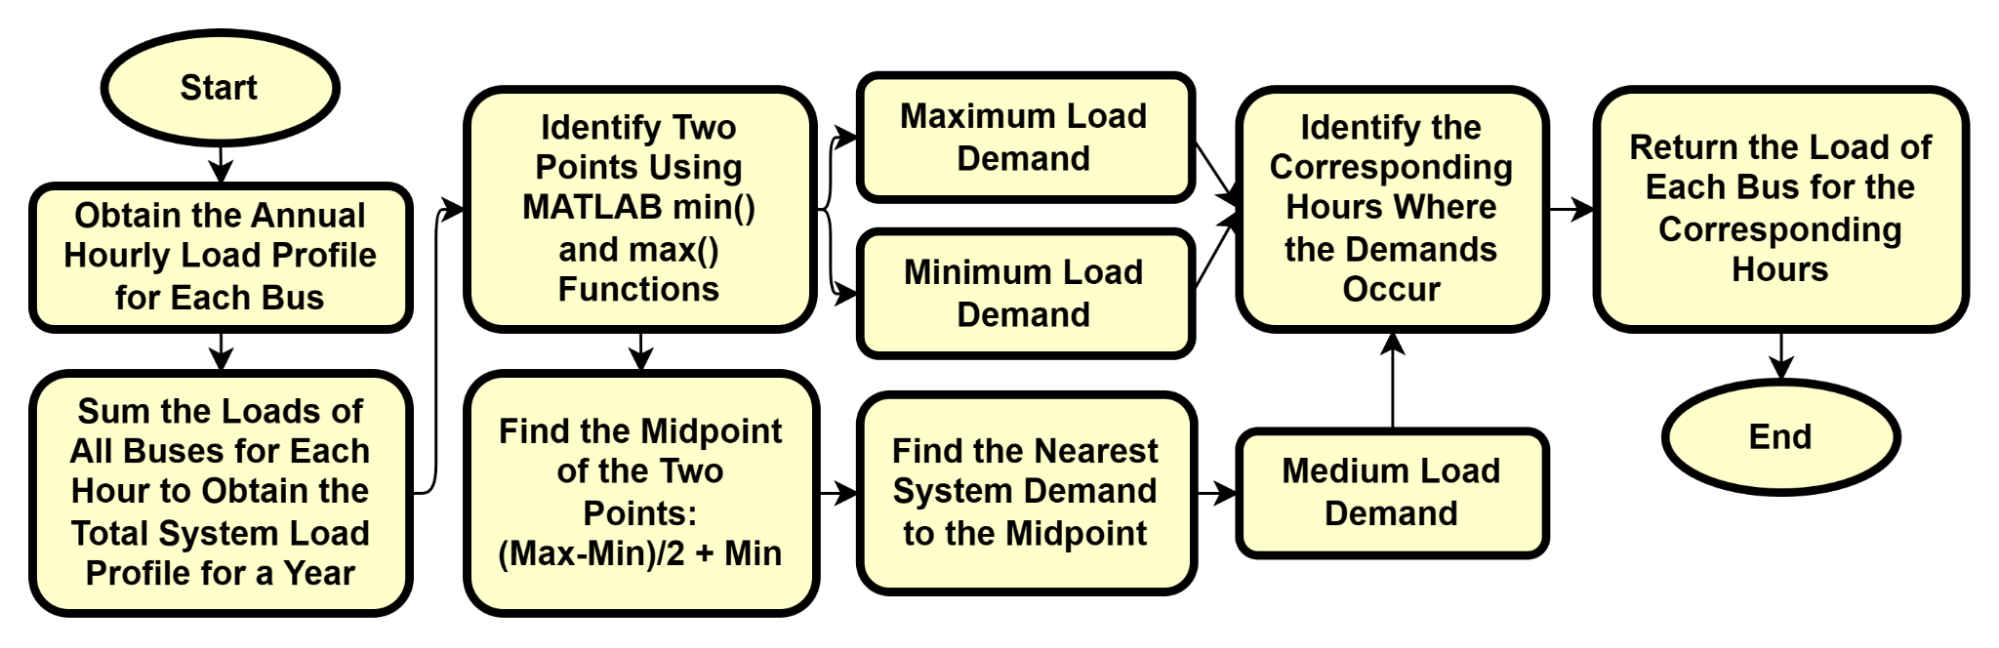
\includegraphics[width=0.5\textwidth]{multilevelflowchart.png}}
%	\caption{3-Hour Load Profile Development Flowchart.}
%	\label{fig:3hourchartdev}
%\end{figure}
%
%
%\begin{table}[htbp]
%	\centering
%	\caption{Load Demand of 33 Buses for 3 Hours}
%	\label{tab:3hoursloadprofile}
%	\resizebox{\columnwidth}{!}{%
%		\begin{tabular}{|c|ccc|ccc|}
%			\hline
%			\textbf{} & \multicolumn{3}{c|}{\textbf{P (kW)}}                                   & \multicolumn{3}{c|}{\textbf{Q (kVAr)}}                                  \\ \hline
%			\textbf{Bus} &
%			\multicolumn{1}{c|}{\textbf{Hour 1}} &
%			\multicolumn{1}{c|}{\textbf{Hour 2}} &
%			\textbf{Hour 3} &
%			\multicolumn{1}{c|}{\textbf{Hour 1}} &
%			\multicolumn{1}{c|}{\textbf{Hour 2}} &
%			\textbf{Hour 3} \\ \hline
%			1         & \multicolumn{1}{c|}{0}       & \multicolumn{1}{c|}{0}       & 0        & \multicolumn{1}{c|}{0}       & \multicolumn{1}{c|}{0}        & 0        \\ \hline
%			2         & \multicolumn{1}{c|}{8.4858}  & \multicolumn{1}{c|}{64.4516} & 96.4926  & \multicolumn{1}{c|}{5.0915}  & \multicolumn{1}{c|}{38.6709}  & 57.8956  \\ \hline
%			3         & \multicolumn{1}{c|}{8.935}   & \multicolumn{1}{c|}{48.282}  & 86.8396  & \multicolumn{1}{c|}{3.9711}  & \multicolumn{1}{c|}{21.4587}  & 38.5954  \\ \hline
%			4         & \multicolumn{1}{c|}{7.8811}  & \multicolumn{1}{c|}{41.2028} & 128.6932 & \multicolumn{1}{c|}{5.2541}  & \multicolumn{1}{c|}{27.4685}  & 85.7955  \\ \hline
%			5         & \multicolumn{1}{c|}{8.5614}  & \multicolumn{1}{c|}{57.998}  & 72.0976  & \multicolumn{1}{c|}{4.2807}  & \multicolumn{1}{c|}{28.999}   & 36.0488  \\ \hline
%			6         & \multicolumn{1}{c|}{7.6754}  & \multicolumn{1}{c|}{57.9392} & 91.2525  & \multicolumn{1}{c|}{2.5585}  & \multicolumn{1}{c|}{19.3131}  & 30.4175  \\ \hline
%			7         & \multicolumn{1}{c|}{8.7167}  & \multicolumn{1}{c|}{44.3225} & 90.7906  & \multicolumn{1}{c|}{4.3584}  & \multicolumn{1}{c|}{22.1613}  & 45.3953  \\ \hline
%			8         & \multicolumn{1}{c|}{13.0079} & \multicolumn{1}{c|}{60.0554} & 82.3049  & \multicolumn{1}{c|}{6.5039}  & \multicolumn{1}{c|}{30.0277}  & 41.1524  \\ \hline
%			9         & \multicolumn{1}{c|}{15.4558} & \multicolumn{1}{c|}{33.7835} & 34.2916  & \multicolumn{1}{c|}{5.1519}  & \multicolumn{1}{c|}{11.2612}  & 11.4305  \\ \hline
%			10        & \multicolumn{1}{c|}{18.101}  & \multicolumn{1}{c|}{42.1559} & 76.0445  & \multicolumn{1}{c|}{6.0337}  & \multicolumn{1}{c|}{14.052}   & 25.3482  \\ \hline
%			11        & \multicolumn{1}{c|}{9.1366}  & \multicolumn{1}{c|}{39.2378} & 87.0537  & \multicolumn{1}{c|}{6.0911}  & \multicolumn{1}{c|}{26.1585}  & 58.0358  \\ \hline
%			12        & \multicolumn{1}{c|}{13.285}  & \multicolumn{1}{c|}{75.9815} & 80.9403  & \multicolumn{1}{c|}{7.7496}  & \multicolumn{1}{c|}{44.3225}  & 47.2151  \\ \hline
%			13        & \multicolumn{1}{c|}{11.828}  & \multicolumn{1}{c|}{47.6354} & 131.4014 & \multicolumn{1}{c|}{6.8997}  & \multicolumn{1}{c|}{27.7873}  & 76.6508  \\ \hline
%			14        & \multicolumn{1}{c|}{11.131}  & \multicolumn{1}{c|}{45.1665} & 73.3362  & \multicolumn{1}{c|}{7.4207}  & \multicolumn{1}{c|}{30.111}   & 48.8908  \\ \hline
%			15        & \multicolumn{1}{c|}{10.1065} & \multicolumn{1}{c|}{35.5092} & 131.4854 & \multicolumn{1}{c|}{1.6844}  & \multicolumn{1}{c|}{5.9182}   & 21.9142  \\ \hline
%			16        & \multicolumn{1}{c|}{12.0086} & \multicolumn{1}{c|}{88.876}  & 97.0594  & \multicolumn{1}{c|}{4.0029}  & \multicolumn{1}{c|}{29.6253}  & 32.3531  \\ \hline
%			17        & \multicolumn{1}{c|}{10.8371} & \multicolumn{1}{c|}{39.1664} & 127.7695 & \multicolumn{1}{c|}{3.6124}  & \multicolumn{1}{c|}{13.0555}  & 42.5898  \\ \hline
%			18        & \multicolumn{1}{c|}{16.9128} & \multicolumn{1}{c|}{62.0792} & 88.2     & \multicolumn{1}{c|}{7.5168}  & \multicolumn{1}{c|}{27.5908}  & 39.2     \\ \hline
%			19        & \multicolumn{1}{c|}{10.4592} & \multicolumn{1}{c|}{51.851}  & 84.7486  & \multicolumn{1}{c|}{4.6485}  & \multicolumn{1}{c|}{23.0449}  & 37.666   \\ \hline
%			20        & \multicolumn{1}{c|}{7.1757}  & \multicolumn{1}{c|}{49.4661} & 67.714   & \multicolumn{1}{c|}{3.1892}  & \multicolumn{1}{c|}{21.9849}  & 30.0951  \\ \hline
%			21        & \multicolumn{1}{c|}{13.1003} & \multicolumn{1}{c|}{48.853}  & 60.2822  & \multicolumn{1}{c|}{5.8223}  & \multicolumn{1}{c|}{21.7125}  & 26.7921  \\ \hline
%			22        & \multicolumn{1}{c|}{9.4095}  & \multicolumn{1}{c|}{62.243}  & 121.2403 & \multicolumn{1}{c|}{4.182}   & \multicolumn{1}{c|}{27.6636}  & 53.8846  \\ \hline
%			23        & \multicolumn{1}{c|}{11.6601} & \multicolumn{1}{c|}{69.3096} & 77.556   & \multicolumn{1}{c|}{6.4778}  & \multicolumn{1}{c|}{38.5053}  & 43.0867  \\ \hline
%			24        & \multicolumn{1}{c|}{14.0828} & \multicolumn{1}{c|}{44.9355} & 184.7052 & \multicolumn{1}{c|}{6.7061}  & \multicolumn{1}{c|}{21.3979}  & 87.9548  \\ \hline
%			25        & \multicolumn{1}{c|}{9.3423}  & \multicolumn{1}{c|}{66.1521} & 82.6492  & \multicolumn{1}{c|}{4.4487}  & \multicolumn{1}{c|}{31.501}   & 39.3567  \\ \hline
%			26        & \multicolumn{1}{c|}{7.2933}  & \multicolumn{1}{c|}{62.2094} & 75.2971  & \multicolumn{1}{c|}{3.0389}  & \multicolumn{1}{c|}{25.9206}  & 31.3738  \\ \hline
%			27        & \multicolumn{1}{c|}{9.2206}  & \multicolumn{1}{c|}{49.0966} & 60.1898  & \multicolumn{1}{c|}{3.8419}  & \multicolumn{1}{c|}{20.4569}  & 25.0791  \\ \hline
%			28        & \multicolumn{1}{c|}{10.1653} & \multicolumn{1}{c|}{42.1266} & 94.2966  & \multicolumn{1}{c|}{3.3884}  & \multicolumn{1}{c|}{14.0422}  & 31.4322  \\ \hline
%			29        & \multicolumn{1}{c|}{11.8322} & \multicolumn{1}{c|}{39.6073} & 93.4653  & \multicolumn{1}{c|}{6.9021}  & \multicolumn{1}{c|}{23.1042}  & 54.5214  \\ \hline
%			30        & \multicolumn{1}{c|}{17.341}  & \multicolumn{1}{c|}{55.6383} & 155.4479 & \multicolumn{1}{c|}{52.0231} & \multicolumn{1}{c|}{166.9149} & 466.3438 \\ \hline
%			31        & \multicolumn{1}{c|}{7.9777}  & \multicolumn{1}{c|}{32.4651} & 110.6761 & \multicolumn{1}{c|}{3.7229}  & \multicolumn{1}{c|}{15.1504}  & 51.6489  \\ \hline
%			32        & \multicolumn{1}{c|}{8.2338}  & \multicolumn{1}{c|}{67.3487} & 77.2579  & \multicolumn{1}{c|}{3.9209}  & \multicolumn{1}{c|}{32.0708}  & 36.7895  \\ \hline
%			33        & \multicolumn{1}{c|}{12.2563} & \multicolumn{1}{c|}{50.8349} & 78.421   & \multicolumn{1}{c|}{8.1709}  & \multicolumn{1}{c|}{33.8899}  & 52.2806  \\ \hline
%		\end{tabular}%
%	}
%\end{table}
%
%\paragraph{Daily Load Demand (24 Hours)}
%The daily load profile consists of 24 hours of load data for the system. To determine this load profile, we first assumed that demand on weekdays and weekends did not differ significantly. Figure~\ref{fig:24hourchartdev} illustrates the process of extracting a representative daily load profile. The detailed load of each bus for 24 hours could be accessed through the supplementary materials titled \href{https://docs.google.com/spreadsheets/d/1aUaok1M9MFdV-2YwGXDtjuIwCXB-yF1H/edit?usp=sharing&ouid=104271507204643812053&rtpof=true&sd=true}{Appendix\_Daily\_Load\_P\_Data.xlsx} and \href{https://docs.google.com/spreadsheets/d/1owMe5SsF_vXdNSdqBIJJ5x3NKYC_CiQ1/edit?usp=sharing&ouid=104271507204643812053&rtpof=true&sd=true}{Appendix\_Daily\_Load\_Q\_Data.xlsx}.
%
%
%\begin{figure}[htbp]
%	\centerline{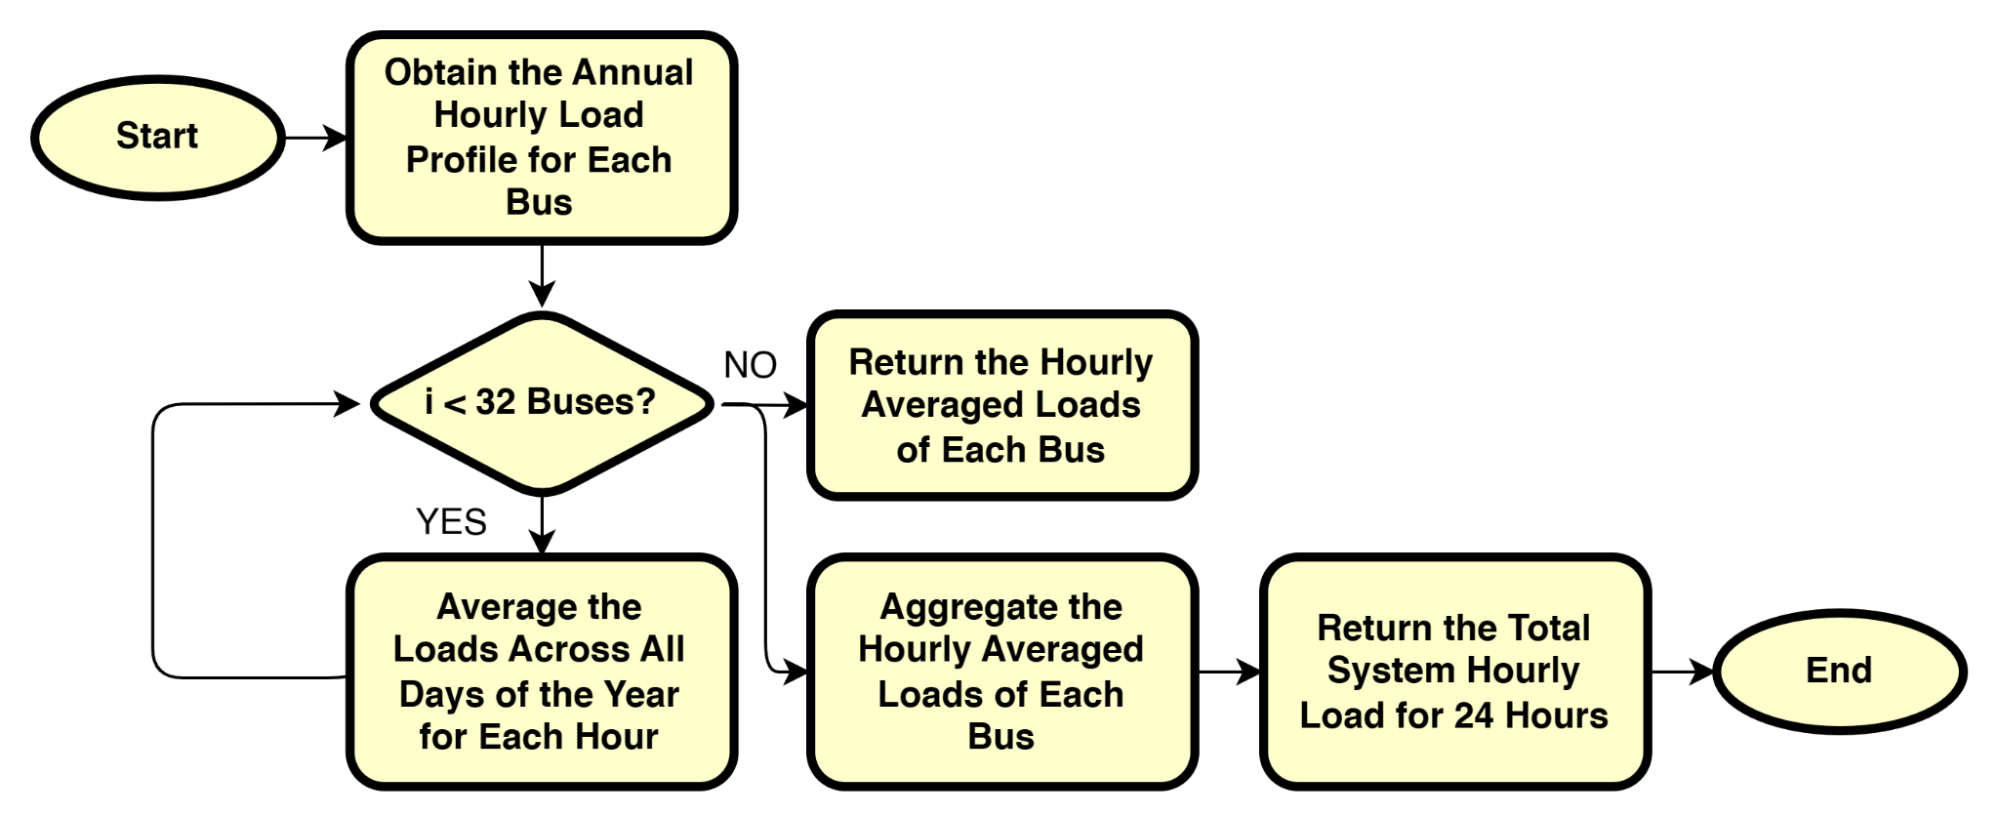
\includegraphics[width=0.5\textwidth]{dailychart.png}}
%	\caption{24-Hour Load Profile Development Flowchart.}
%	\label{fig:24hourchartdev}
%\end{figure}
%
%
%\paragraph{Seasonal Load Demand (96 Hours)}
%We condensed four seasons into a 96-hour load profile, where each season is represented in a 24-hour period. Figure \ref{fig:96hourchartdev} provides an illustration of how the seasonal load profiles are developed. The detailed load of each bus for 96 hours could be accessed through the supplementary materials titled \href{https://docs.google.com/spreadsheets/d/1aUaok1M9MFdV-2YwGXDtjuIwCXB-yF1H/edit?usp=sharing&ouid=104271507204643812053&rtpof=true&sd=true}{Appendix\_Seasonal\_Load\_P\_Data.xlsx} and \href{https://docs.google.com/spreadsheets/d/12WRgx53A4gAkal306UHPLYaDwVpHLaF3/edit?usp=sharing&ouid=104271507204643812053&rtpof=true&sd=true}{Appendix\_Seasonal\_Load\_Q\_Data.xlsx}.
%
%\begin{figure}[htbp]
%	\centerline{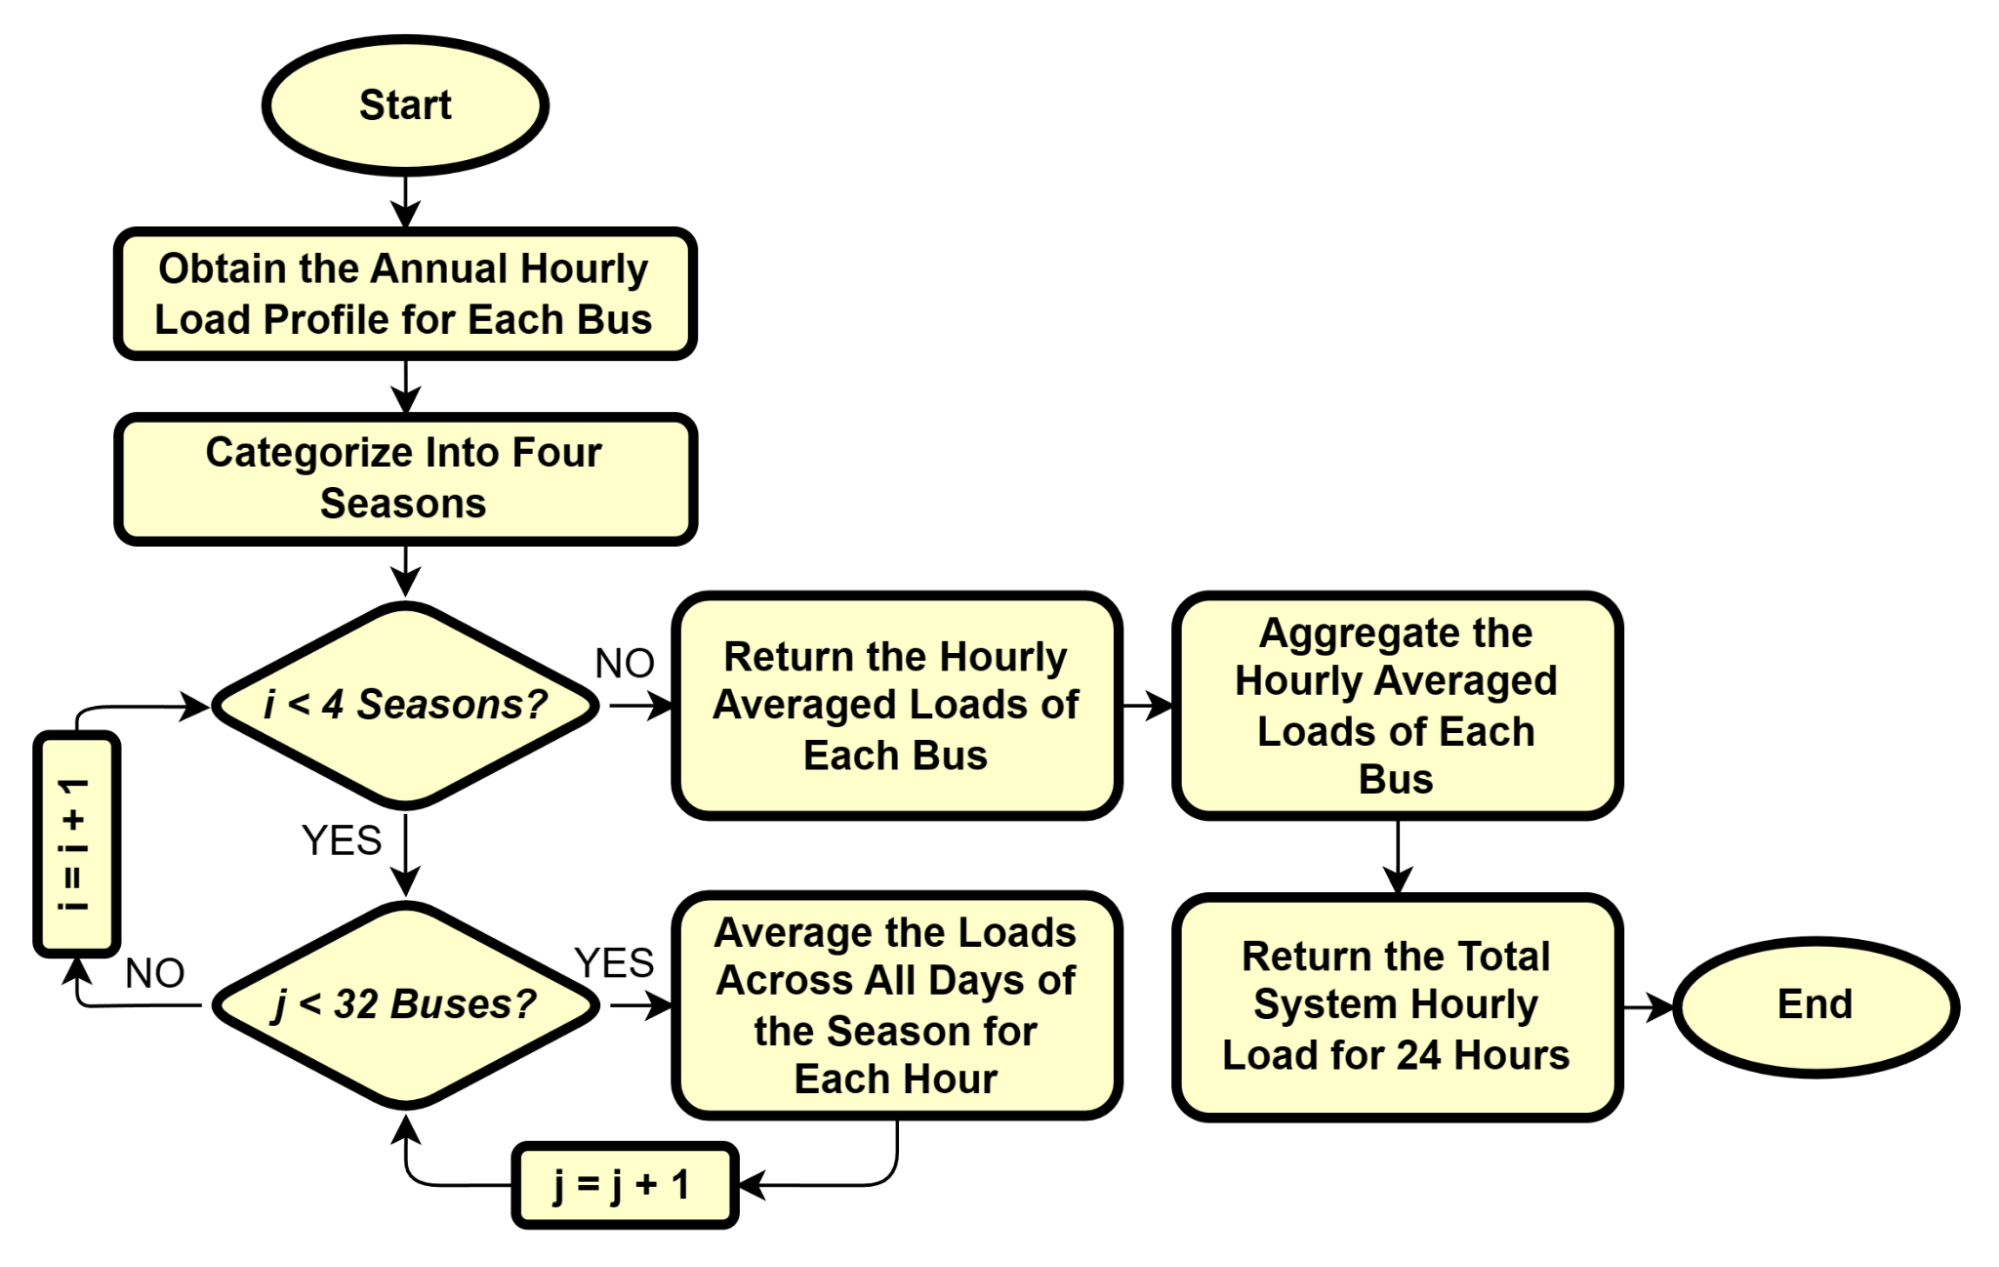
\includegraphics[width=0.5\textwidth]{96hourchart.png}}
%	\caption{96-Hour Load Profile Development Flowchart.}
%	\label{fig:96hourchartdev}
%\end{figure}
%
%\subsection{Results Data}
%This section details the bus and line data used in the study.
%
%\subsubsection{Comparison of Published Results For Single DG Integration}
%
%Table~\ref{tab:singleDGcomparison} presents the optimal allocation of a DG with the corresponding power losses from studies conducted until 2016. Results indicate that both WOA and E-WOA are effective optimizers for this problem.
%
%\begin{table}[htbp]
%	\caption{Optimization Results for Single DG in IEEE 33-Bus System at Unity Power Factor}
%%	\vspace{-20pt}
%	\begin{center}
%		\resizebox{\columnwidth}{!}{%
%			\begin{tabular}{ccccc}
%				\hline
%				\textbf{Year} &
%				\textbf{Algorithm} &
%				\textbf{\begin{tabular}[c]{@{}c@{}}DG \\ Location\end{tabular}} &
%				\textbf{\begin{tabular}[c]{@{}c@{}}DG Size\\  (kW)\end{tabular}} &
%				\textbf{Power Loss (kW)} \\ \hline
%				\multicolumn{2}{c}{Base}             & -          & -                 & 210.988          \\
%				2016$^{\mathrm{a}}$             & BFOA           & 6          & 2200.000          & 113.140          \\
%				2016$^{\mathrm{b}}$            & HSA-PABC       & 6          & 2598.000          & 111.030          \\
%				2017$^{\mathrm{c}}$            & GWO            & 6          & 2761.820          & 111.420          \\
%				2018$^{\mathrm{d}}$             & GA             & 6          & 2600.000          & 111.030          \\
%				2018$^{\mathrm{e}}$             & DA             & 6          & 2590.200          & 111.034          \\
%				2021$^{\mathrm{f}}$            & MRFO           & 6          & 2590.217          & 111.027          \\
%				2021$^{\mathrm{g}}$            & PFA            & 6          & 2590.264          & 111.030          \\
%				2022$^{\mathrm{h}}$             & HBA            & 30         & 1542.000          & 125.000          \\
%				\textbf{Present} & \textbf{WOA}   & \textbf{6} & \textbf{2590.217} & \textbf{111.019} \\
%				\textbf{Present} & \textbf{E-WOA} & \textbf{6} & \textbf{2590.217} & \textbf{111.019} \\ \hline
%				\multicolumn{5}{l}{$^{\mathrm{a}}${\scriptsize Devabalaji et al., 2016.}} \\
%				\multicolumn{5}{l}{$^{\mathrm{b}}${\scriptsize Muthukumar et al., 2016.}} \\
%				\multicolumn{5}{l}{$^{\mathrm{c}}${\scriptsize El-Sayed et al., 2017.}} \\
%				\multicolumn{5}{l}{$^{\mathrm{d}}${\scriptsize Kashyap et al., 2018.}} \\
%				\multicolumn{5}{l}{$^{\mathrm{e}}${\scriptsize Suresh et al., 2018.}} \\
%				\multicolumn{5}{l}{$^{\mathrm{f}}${\scriptsize Hemeida et al., 2021.}} \\
%				\multicolumn{5}{l}{$^{\mathrm{g}}${\scriptsize Janamala, 2021.}} \\
%				\multicolumn{5}{l}{$^{\mathrm{h}}${\scriptsize Khan, 2022.}} \\
%			\end{tabular}%
%		}
%		\label{tab:singleDGcomparison}
%	\end{center}
%\end{table}
%
%\subsubsection{Optimization Algorithm}
%\paragraph{Whale Optimization Algorithm (WOA)}
%
%Fig. \ref{fig:WOAflowchart} presents the optimal flowchart of WOA including the modifications implemented for solving the mixed-integer ODGA problem.
%
%\begin{figure}[htbp]
%	\centerline{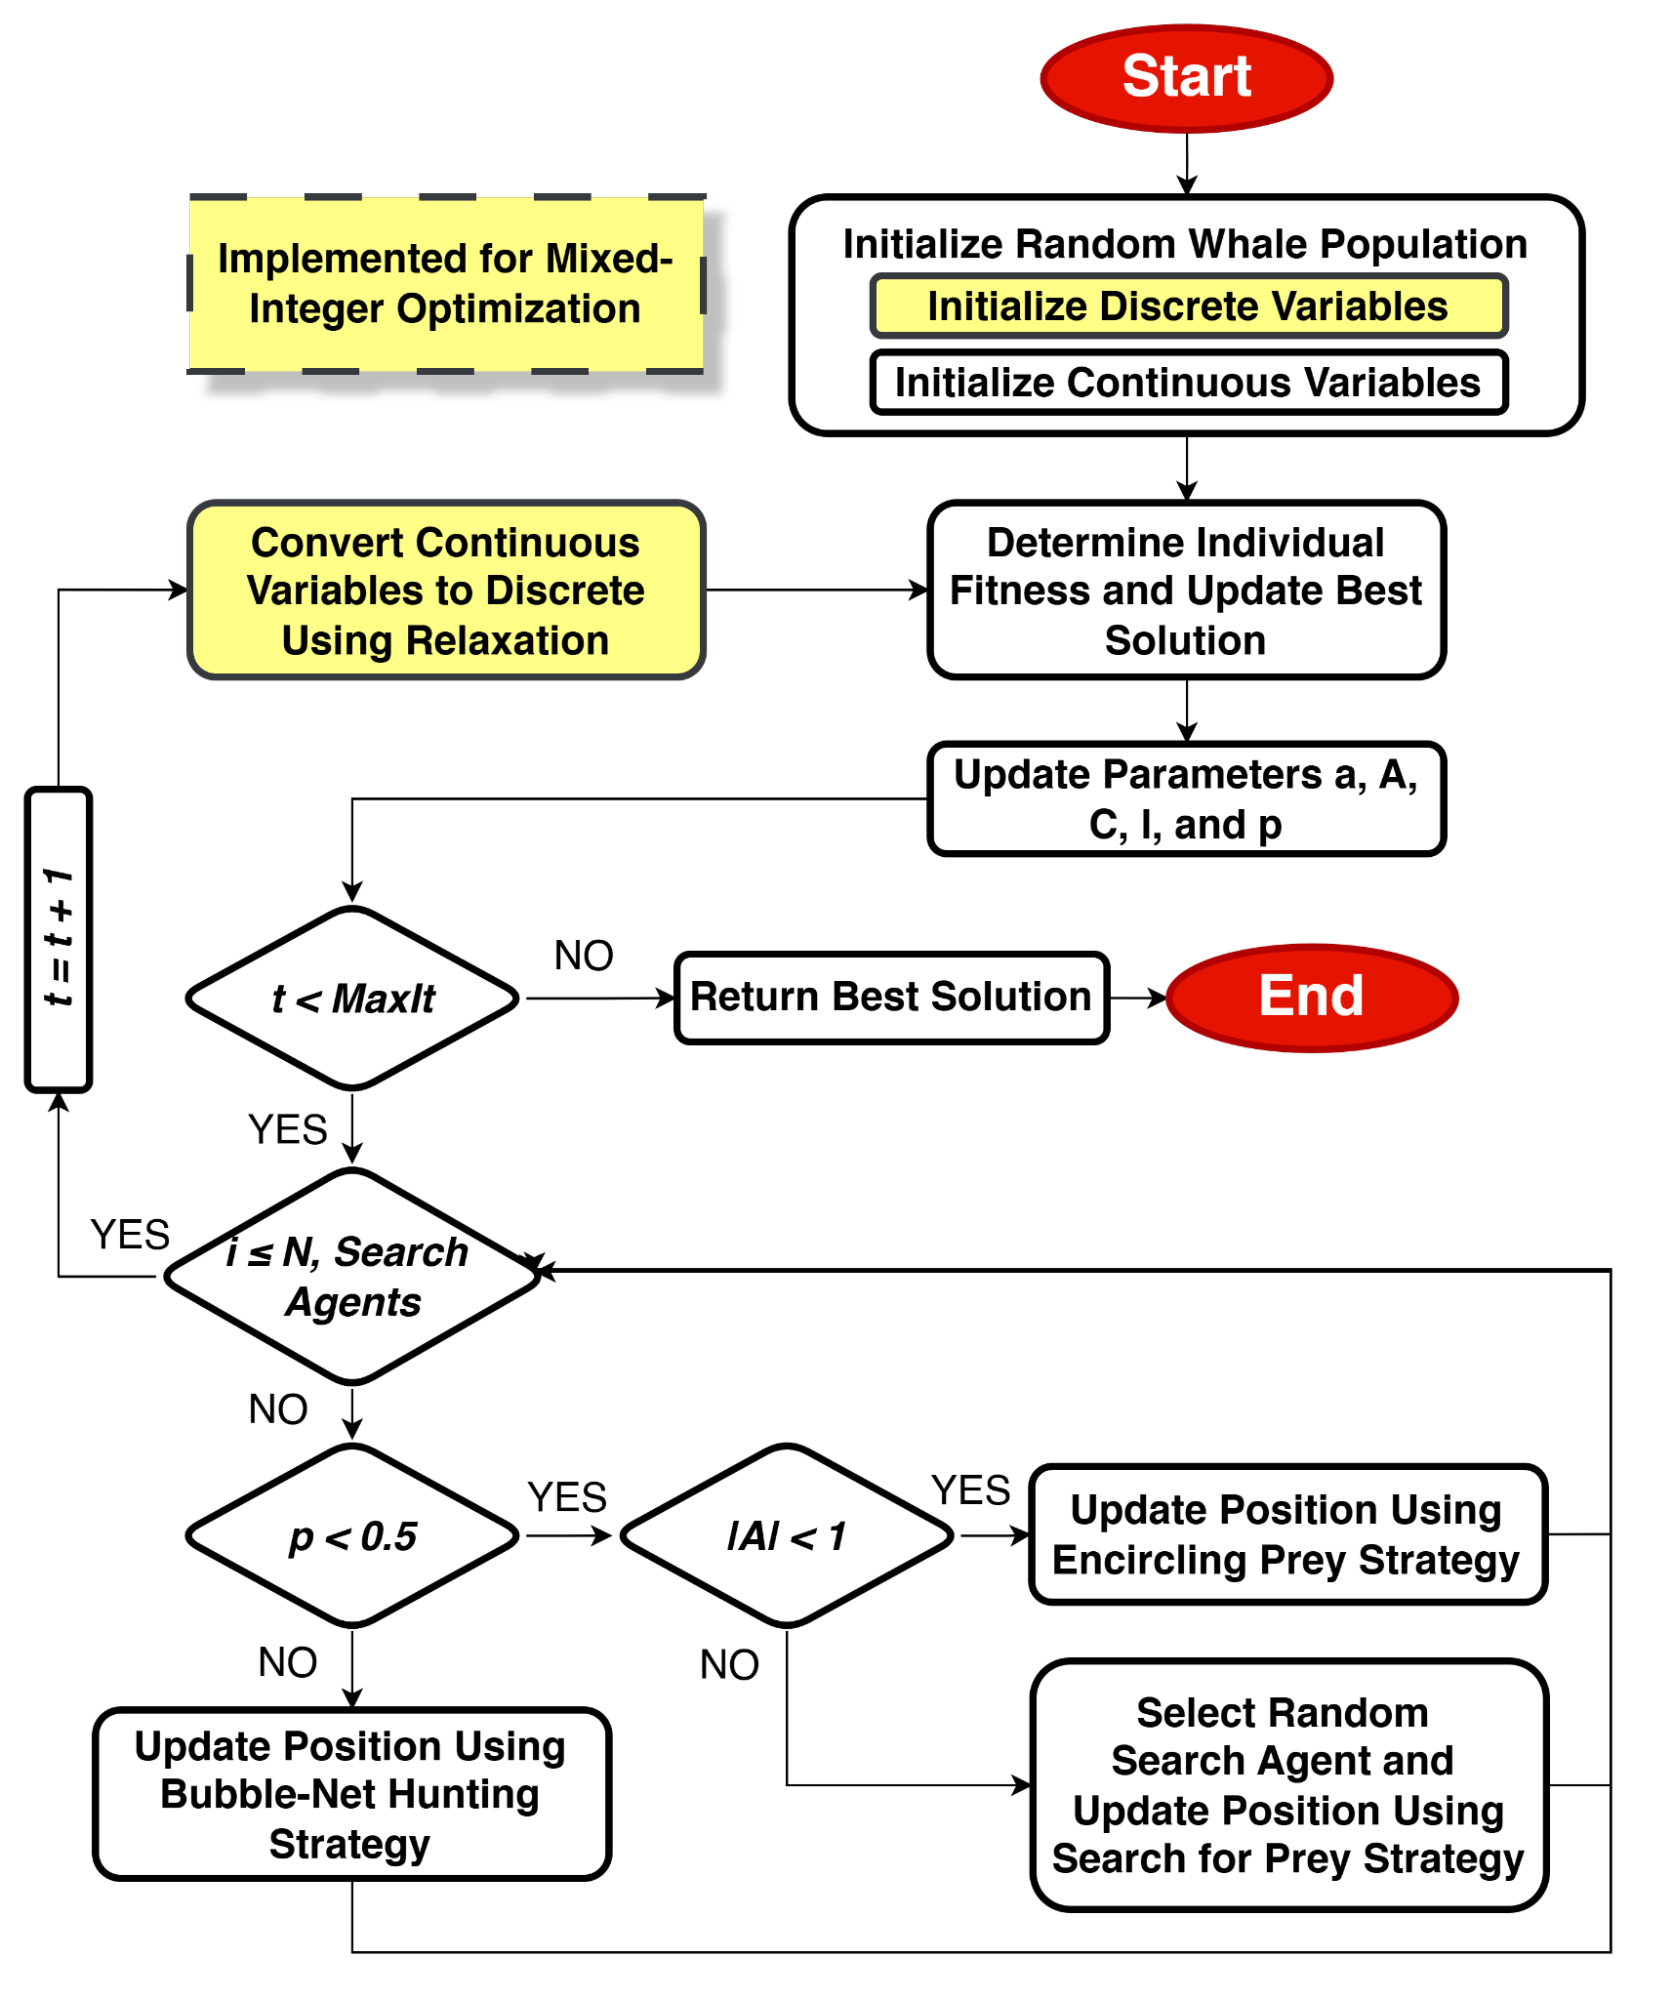
\includegraphics[width=0.5\textwidth]{WOAflowchart.png}}
%	\caption{24-Hour Load Profile Development Flowchart.}
%	\label{fig:WOAflowchart}
%\end{figure}
%
%\subsubsection{Convergence Curves}
%The following figures illustrate the convergence curves of WOA and E-WOA for 100 runs as well as the comparison of their best convergence curves.
%
%
%\paragraph{Case 1 Comparison}
%
%Fig. \ref{fig:case1convcomp} presents the comparison of the best convergence curve of each algorithm for Case 1.
%
%\begin{figure}[htbp]
%	\centerline{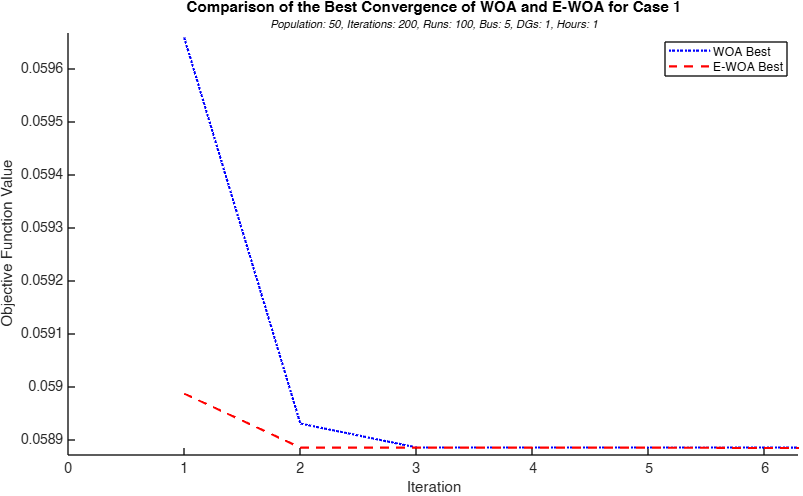
\includegraphics[width=0.5\textwidth]{case1comp.png}}
%	\caption{Comparison of Best Convergence Curves for Case 1.}
%	\label{fig:case1convcomp}
%\end{figure}
%
%\paragraph{Case 2 Comparison}
%
%Fig. \ref{fig:case2convcomp} presents the comparison of the best convergence curve of each algorithm for Case 2.
%
%\begin{figure}[htbp]
%	\centerline{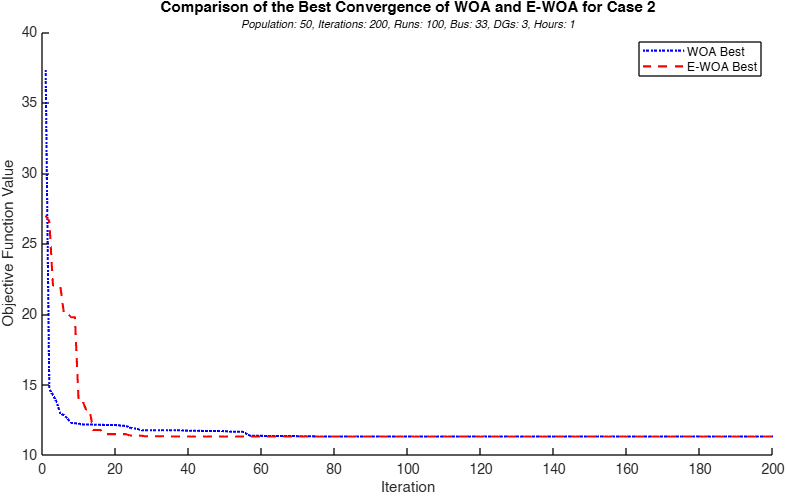
\includegraphics[width=0.5\textwidth]{case2comp.png}}
%	\caption{Comparison of Best Convergence Curves for Case 2.}
%	\label{fig:case2convcomp}
%\end{figure}
%
%\paragraph{Case 3 Comparison}
%
%Fig. \ref{fig:case3convcomp} presents the comparison of the best convergence curve of each algorithm for Case 3.
%
%\begin{figure}[htbp]
%	\centerline{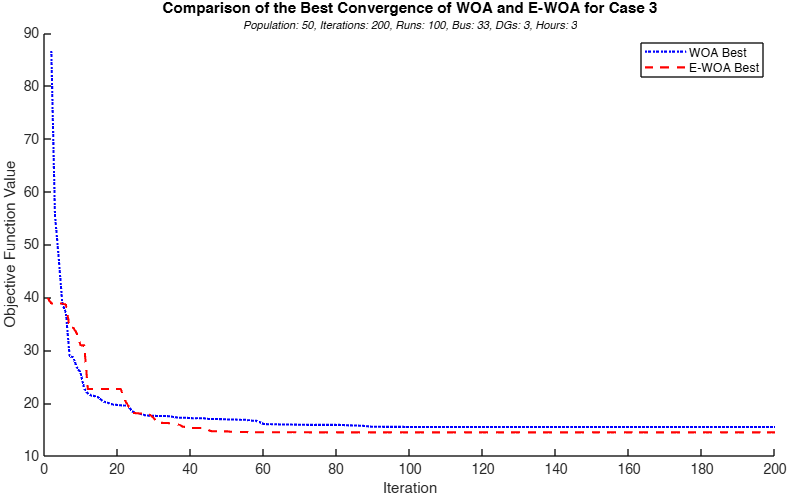
\includegraphics[width=0.5\textwidth]{case3comp.png}}
%	\caption{Comparison of Best Convergence Curves for Case 3.}
%	\label{fig:case3convcomp}
%\end{figure}
%
%\paragraph{Case 5 Comparison}
%
%Fig. \ref{fig:case5convcomp} presents the comparison of the best convergence curve of each algorithm for Case 5. Since E-WOA failed to find any feasible solutions in 100 runs, only WOA's convergence curve is shown.
%
%\begin{figure}[htbp]
%	\centerline{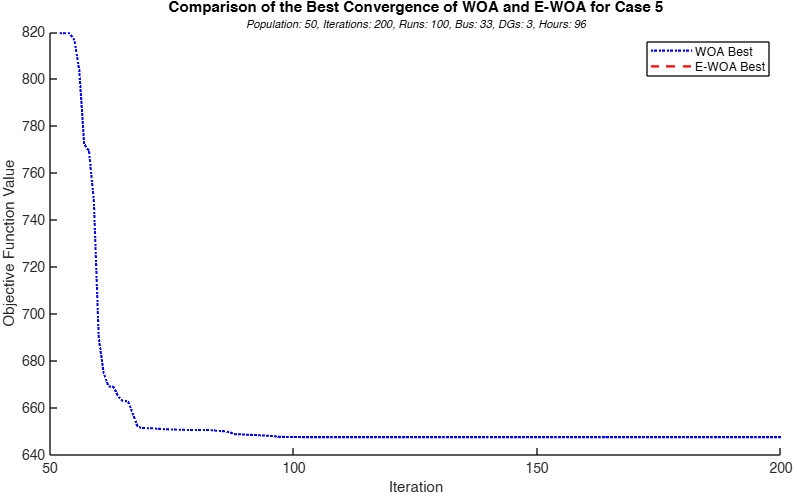
\includegraphics[width=0.5\textwidth]{case5comp.png}}
%	\caption{Comparison of Best Convergence Curves for Case 5.}
%	\label{fig:case5convcomp}
%\end{figure}
%
%
%
%
%
%
%
%%\multicolumn{7}{l}{$^{\mathrm{a}}${\scriptsize I.w.V. is Iterations with Violations.}} \\
%%$^{\mathrm{a}}$
%%
%%\vspace{100pt}
%%
%%\section{Prepare Your Paper Before Styling}
%%Before you begin to format your paper, first write and save the content as a 
%%separate text file. Complete all content and organizational editing before 
%%formatting. Please note sections \ref{AA}--\ref{SCM} below for more information on 
%%proofreading, spelling and grammar.
%%
%%Keep your text and graphic files separate until after the text has been 
%%formatted and styled. Do not number text heads---{\LaTeX} will do that 
%%for you.
%%
%%\subsection{Abbreviations and Acronyms}\label{AA}
%%Define abbreviations and acronyms the first time they are used in the text, 
%%even after they have been defined in the abstract. Abbreviations such as 
%%IEEE, SI, MKS, CGS, ac, dc, and rms do not have to be defined. Do not use 
%%abbreviations in the title or heads unless they are unavoidable.
%%
%%\subsection{Units}
%%\begin{itemize}
%%	\item Use either SI (MKS) or CGS as primary units. (SI units are encouraged.) English units may be used as secondary units (in parentheses). An exception would be the use of English units as identifiers in trade, such as ``3.5-inch disk drive''.
%%	\item Avoid combining SI and CGS units, such as current in amperes and magnetic field in oersteds. This often leads to confusion because equations do not balance dimensionally. If you must use mixed units, clearly state the units for each quantity that you use in an equation.
%%	\item Do not mix complete spellings and abbreviations of units: ``Wb/m\textsuperscript{2}'' or ``webers per square meter'', not ``webers/m\textsuperscript{2}''. Spell out units when they appear in text: ``. . . a few henries'', not ``. . . a few H''.
%%	\item Use a zero before decimal points: ``0.25'', not ``.25''. Use ``cm\textsuperscript{3}'', not ``cc''.)
%%\end{itemize}
%%
%%\subsection{Equations}
%%Number equations consecutively. To make your 
%%equations more compact, you may use the solidus (~/~), the exp function, or 
%%appropriate exponents. Italicize Roman symbols for quantities and variables, 
%%but not Greek symbols. Use a long dash rather than a hyphen for a minus 
%%sign. Punctuate equations with commas or periods when they are part of a 
%%sentence, as in:
%%\begin{equation}
%%	a+b=\gamma\label{eq}
%%\end{equation}
%%
%%Be sure that the 
%%symbols in your equation have been defined before or immediately following 
%%the equation. Use ``\eqref{eq}'', not ``Eq.~\eqref{eq}'' or ``equation \eqref{eq}'', except at 
%%the beginning of a sentence: ``Equation \eqref{eq} is . . .''
%%
%%\subsection{\LaTeX-Specific Advice}
%%
%%Please use ``soft'' (e.g., \verb|\eqref{Eq}|) cross references instead
%%of ``hard'' references (e.g., \verb|(1)|). That will make it possible
%%to combine sections, add equations, or change the order of figures or
%%citations without having to go through the file line by line.
%%
%%Please don't use the \verb|{eqnarray}| equation environment. Use
%%\verb|{align}| or \verb|{IEEEeqnarray}| instead. The \verb|{eqnarray}|
%%environment leaves unsightly spaces around relation symbols.
%%
%%Please note that the \verb|{subequations}| environment in {\LaTeX}
%%will increment the main equation counter even when there are no
%%equation numbers displayed. If you forget that, you might write an
%%article in which the equation numbers skip from (17) to (20), causing
%%the copy editors to wonder if you've discovered a new method of
%%counting.
%%
%%{\BibTeX} does not work by magic. It doesn't get the bibliographic
%%data from thin air but from .bib files. If you use {\BibTeX} to produce a
%%bibliography you must send the .bib files. 
%%
%%{\LaTeX} can't read your mind. If you assign the same label to a
%%subsubsection and a table, you might find that Table I has been cross
%%referenced as Table IV-B3. 
%%
%%{\LaTeX} does not have precognitive abilities. If you put a
%%\verb|\label| command before the command that updates the counter it's
%%supposed to be using, the label will pick up the last counter to be
%%cross referenced instead. In particular, a \verb|\label| command
%%should not go before the caption of a figure or a table.
%%
%%Do not use \verb|\nonumber| inside the \verb|{array}| environment. It
%%will not stop equation numbers inside \verb|{array}| (there won't be
%%any anyway) and it might stop a wanted equation number in the
%%surrounding equation.
%%
%%\subsection{Some Common Mistakes}\label{SCM}
%%\begin{itemize}
%%	\item The word ``data'' is plural, not singular.
%%	\item The subscript for the permeability of vacuum $\mu_{0}$, and other common scientific constants, is zero with subscript formatting, not a lowercase letter ``o''.
%%	\item In American English, commas, semicolons, periods, question and exclamation marks are located within quotation marks only when a complete thought or name is cited, such as a title or full quotation. When quotation marks are used, instead of a bold or italic typeface, to highlight a word or phrase, punctuation should appear outside of the quotation marks. A parenthetical phrase or statement at the end of a sentence is punctuated outside of the closing parenthesis (like this). (A parenthetical sentence is punctuated within the parentheses.)
%%	\item A graph within a graph is an ``inset'', not an ``insert''. The word alternatively is preferred to the word ``alternately'' (unless you really mean something that alternates).
%%	\item Do not use the word ``essentially'' to mean ``approximately'' or ``effectively''.
%%	\item In your paper title, if the words ``that uses'' can accurately replace the word ``using'', capitalize the ``u''; if not, keep using lower-cased.
%%	\item Be aware of the different meanings of the homophones ``affect'' and ``effect'', ``complement'' and ``compliment'', ``discreet'' and ``discrete'', ``principal'' and ``principle''.
%%	\item Do not confuse ``imply'' and ``infer''.
%%	\item The prefix ``non'' is not a word; it should be joined to the word it modifies, usually without a hyphen.
%%	\item There is no period after the ``et'' in the Latin abbreviation ``et al.''.
%%	\item The abbreviation ``i.e.'' means ``that is'', and the abbreviation ``e.g.'' means ``for example''.
%%\end{itemize}
%%An excellent style manual for science writers is \cite{b7}.
%%
%%\subsection{Authors and Affiliations}
%%\textbf{The class file is designed for, but not limited to, six authors.} A 
%%minimum of one author is required for all conference articles. Author names 
%%should be listed starting from left to right and then moving down to the 
%%next line. This is the author sequence that will be used in future citations 
%%and by indexing services. Names should not be listed in columns nor group by 
%%affiliation. Please keep your affiliations as succinct as possible (for 
%%example, do not differentiate among departments of the same organization).
%%
%%\subsection{Identify the Headings}
%%Headings, or heads, are organizational devices that guide the reader through 
%%your paper. There are two types: component heads and text heads.
%%
%%Component heads identify the different components of your paper and are not 
%%topically subordinate to each other. Examples include Acknowledgments and 
%%References and, for these, the correct style to use is ``Heading 5''. Use 
%%``figure caption'' for your Figure captions, and ``table head'' for your 
%%table title. Run-in heads, such as ``Abstract'', will require you to apply a 
%%style (in this case, italic) in addition to the style provided by the drop 
%%down menu to differentiate the head from the text.
%%
%%Text heads organize the topics on a relational, hierarchical basis. For 
%%example, the paper title is the primary text head because all subsequent 
%%material relates and elaborates on this one topic. If there are two or more 
%%sub-topics, the next level head (uppercase Roman numerals) should be used 
%%and, conversely, if there are not at least two sub-topics, then no subheads 
%%should be introduced.
%%
%%\subsection{Figures and Tables}
%%\paragraph{Positioning Figures and Tables} Place figures and tables at the top and 
%%bottom of columns. Avoid placing them in the middle of columns. Large 
%%figures and tables may span across both columns. Figure captions should be 
%%below the figures; table heads should appear above the tables. Insert 
%%figures and tables after they are cited in the text. Use the abbreviation 
%%``Fig.~\ref{fig}'', even at the beginning of a sentence.
%%
%%\begin{table}[htbp]
%%	\caption{Table Type Styles}
%%	\begin{center}
%%		\begin{tabular}{|c|c|c|c|}
%%			\hline
%%			\textbf{Table}&\multicolumn{3}{|c|}{\textbf{Table Column Head}} \\
%%			\cline{2-4} 
%%			\textbf{Head} & \textbf{\textit{Table column subhead}}& \textbf{\textit{Subhead}}& \textbf{\textit{Subhead}} \\
%%			\hline
%%			copy& More table copy$^{\mathrm{a}}$& &  \\
%%			\hline
%%			\multicolumn{4}{l}{$^{\mathrm{a}}$Sample of a Table footnote.}
%%		\end{tabular}
%%		\label{tab1}
%%	\end{center}
%%\end{table}
%%
%%\begin{figure}[htbp]
%%	\centerline{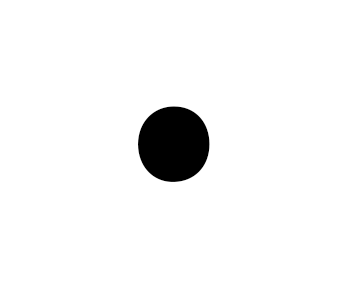
\includegraphics{fig1.png}}
%%	\caption{Example of a figure caption.}
%%	\label{fig}
%%\end{figure}
%%
%%Figure Labels: Use 8 point Times New Roman for Figure labels. Use words 
%%rather than symbols or abbreviations when writing Figure axis labels to 
%%avoid confusing the reader. As an example, write the quantity 
%%``Magnetization'', or ``Magnetization, M'', not just ``M''. If including 
%%units in the label, present them within parentheses. Do not label axes only 
%%with units. In the example, write ``Magnetization (A/m)'' or ``Magnetization 
%%\{A[m(1)]\}'', not just ``A/m''. Do not label axes with a ratio of 
%%quantities and units. For example, write ``Temperature (K)'', not 
%%``Temperature/K''.
%%
%%\section*{Acknowledgment}
%%
%%The preferred spelling of the word ``acknowledgment'' in America is without 
%%an ``e'' after the ``g''. Avoid the stilted expression ``one of us (R. B. 
%%G.) thanks $\ldots$''. Instead, try ``R. B. G. thanks$\ldots$''. Put sponsor 
%%acknowledgments in the unnumbered footnote on the first page.

\end{document}
